%%%%%%%%%%%%%%%%%%%%%%%%%%% asme2ej.tex %%%%%%%%%%%%%%%%%%%%%%%%%%%%%%%
% Template for producing ASME-format journal articles using LaTeX    %
% Written by   Harry H. Cheng, Professor and Director                %
%              Integration Engineering Laboratory                    %
%              Department of Mechanical and Aeronautical Engineering %
%              University of California                              %
%              Davis, CA 95616                                       %
%              Tel: (530) 752-5020 (office)                          %
%                   (530) 752-1028 (lab)                             %
%              Fax: (530) 752-4158                                   %
%              Email: hhcheng@ucdavis.edu                            %
%              WWW:   http://iel.ucdavis.edu/people/cheng.html       %
%              May 7, 1994                                           %
% Modified: February 16, 2001 by Harry H. Cheng                      %
% Modified: January  01, 2003 by Geoffrey R. Shiflett                %
% Use at your own risk, send complaints to /dev/null                 %
%%%%%%%%%%%%%%%%%%%%%%%%%%%%%%%%%%%%%%%%%%%%%%%%%%%%%%%%%%%%%%%%%%%%%%

%%% use twocolumn and 10pt options with the asme2ej format
\documentclass[onecolumn,10pt,final]{asme2ej}

\usepackage{graphicx} %% for loading postscript figures
\usepackage{ctable}
\usepackage{multirow}
\usepackage{colortbl}
\usepackage{amsmath}
\usepackage{amsfonts}
\usepackage{amssymb}


%% The class has several options
%  onecolumn/twocolumn - format for one or two columns per page
%  10pt/11pt/12pt - use 10, 11, or 12 point font
%  oneside/twoside - format for oneside/twosided printing
%  final/draft - format for final/draft copy
%  cleanfoot - take out copyright info in footer leave page number
%  cleanhead - take out the conference banner on the title page
%  titlepage/notitlepage - put in titlepage or leave out titlepage
%  
%% The default is oneside, onecolumn, 10pt, final


\title{An Automatic Switching Approach to Teleoperation of Mobile-Manipulator Systems Using Virtual Fixtures}

%%% first author
\author{M R Wrock
    \affiliation{
	Mechatronic and Robotic Systems Laboratory\\
	University of Ontario: Institute of Technology\\
	Oshawa, Canada\\
    Email: michael.wrock@uoit.ca
    }	
}

%%% second author
%%% remove the following entry for single author papers
%%% add more entries for additional authors
\author{S B Nokleby \\
    \affiliation{
	Mechatronic and Robotic Systems Laboratory\\
	University of Ontario: Institute of Technology\\
	Oshawa, Canada\\
    Email: scott.nokleby@uoit.ca
    }
}

\begin{document}

\maketitle    

%%%%%%%%%%%%%%%%%%%%%%%%%%%%%%%%%%%%%%%%%%%%%%%%%%%%%%%%%%%%%%%%%%%%%%
\begin{abstract}
{\it This work presents a novel command strategy developed to improve operator performance and minimize difficulties in teleoperation tasks for mobile-manipulator systems with a holonomic base. Aimed specifically at novice operators, virtual fixtures are introduced as a means to minimize collisions and assist in navigation. Using the six degree-of-freedom (DOF) Omnibot mobile-manipulator system, a command strategy is implemented such that the operator need only control a three degree-of-freedom haptic joystick to achieve full control of the Omnibot Mobile-Manipulator System (MMS). The command strategy is used to coordinate control between the arm and the base of the system, prevent collisions with known obstacles, and alert the operator of proximity to those obstacles with haptic forces. Through experimental testing it is shown that operator performance improved with the use of virtual fixtures.
}
\end{abstract}

%%%%%%%%%%%%%%%%%%%%%%%%%%%%%%%%

\section{Introduction}
\label{sec:theothersection}
Teleoperation is a process in which an operator controls a robotic system from a remote location. In some cases the robot is in the same room as the operator while in other cases the operator is located in another country or continent and uses a communication protocol via an internet connection to achieve teleoperation  \cite{WangD}. Near or far, teleoperation has uses in medical fields\cite{Diy}, industrial applications\cite{Diy2}, and civil service\cite{kron}. There are many benefits of using a teleoperated robot in place of a human being. Robots can be stronger as well as much larger or smaller than humans, allowing a person to perform tasks that would otherwise be impossible to do alone\cite{j}. They can be used as an assistive device for a disabled person allowing them freedom to perform everyday tasks they would normally require an assistant for\cite{Palankar}. Since robots can be more accurate and precise than a human, they are ideal for delicate manipulation tasks like microsurgery\cite{melch}. Through the use of teleoperation, many surgical procedures can be done from remote locations, anywhere in the world\cite{Diy3}. Robots are often used when there is risk to human life such as radioactive or otherwise toxic environments, bomb diffusal, or search and rescue in potentially dangerous settings.\\

With recent advancements in sensing and processing technologies many robots are able to perform tasks autonomously, but robot Artificial Intelligence (AI) has not reached a point where it can replace a human's reasoning and problem solving ability. For that reason there is a need for robot teleoperation, and with teleoperation comes the requirement for a command strategy. The command strategy dictates how the robot will behave given the operator's commands. Teleoperation is most commonly employed on Mobile-Manipulator Systems (MMS) because it gives the operator the functionality of a fixed manipulator and the mobility of a mobile robot. Most MMS consist of a robotic manipulator, often in a serial configuration. Since the manipulator mimics both the form and function of a human arm, the manipulator portion of a MMS is nicknamed the ``arm''. The part of the MMS that allows locomotion is called the ``base'' and is used to reposition the arm by driving (or otherwise moving) to a desired location.\\

The command strategies for teleoperating robots vary in style and implementation as much as the robots themselves do. The simplest command strategy is for the operator to control each degree-of-freedom (DOF) individually. While simple with regards to the command strategy, this is probably the most difficult way to operate a MMS as it requires a great deal of training and experience for each type of MMS. One common approach to simplify control of a MMS is to view it as an optimization problem, where the operator defines a pose or trajectory and either the base, arm, or both parts of the MMS move according to predefined optimization criteria\cite{yasuaki}. The optimization approach becomes increasingly complex with additional redundant DOF. A MMS is considered redundant if it has more DOF than is required to perform a given task. If said task simply requires position and orientation, the necessary DOF is six, and therefore if a 6-DOF manipulator is used with a 3-DOF base the MMS has three redundant DOF. When viewed as a redundancy resolution problem there is a great deal of literature discussing how to solve redundancy, since redundancy resolution has been a topic of discussion well before the advent of MMS.\\

Since redundancy resolution is a mature field of research, there are many solutions for redundancy in the literature. One example is using additional task constraints so that the system can only find a single configuration for the desired pose (position and orientation). There are many constraints that can be added to a redundant system to minimize the number of solutions to a given motion or pose. A few of these constraints are impedance control\cite{yamanaka}; arm/elbow angle control \cite{equip}, base positioning, collision avoidance\cite{lim}; workspace limits\cite{shin}; singularity avoidance\cite{chung}; sub-task objectives\cite{nath}; configuration control\cite{a}; or multi-criteria optimization\cite{pin}. Additional task constraints are used to make a redundant robot's Jacobian matrix square and thus invertible. A Jacobian matrix is a system of equations used to calculate the velocity of the end-effector based on the joint velocities of the manipulator. Most often, the operator desires to control the motion of the end-effector and the control system is required to determine the appropriate joint velocities based on the operator's commands. To calculate the required joint velocities, the control system must use the inverse of the Jacobian matrix. In the case of a redundant manipulator the Jacobian is not square and requires additional task constraints to be inverted. There are alternatives to additional task constraints to invert a Jacobian matrix such as the Moore-Penrose pseudo-inverse\cite{dir7}, Shamir and Yomdin's modified Moore-Penrose pseudo-inverse for repeatability\cite{dir10}, transpose-based solutions\cite{dir12}, augmented task space\cite{dir18}, extended Jacobian\cite{dir19}, and modified forms of the extended Jacobian\cite{dir22}. There are many different ways of solving the system of equations of motion, but most have significant drawbacks. Whereas some solutions provide a perfectly acceptable solution on paper, they are not ideal when implemented. A major drawback is that many solutions are not singularity robust. When a robot reaches a singularity it loses one or more DOF, leading to lowered manipulability. As well, in some cases as a manipulator approaches a singularity one or more of its joint velocities may approach impractically high values. Singularities are usually avoided, or at the least solutions are sought in which the command strategy can decide when to use singular configurations or not. Aside from the kinematic singularities mentioned the algorithm for solving the equations of motion are prone to algorithmic singularities as well, which would be unacceptable in actual implementation. In the past a significant limitation of using these redundancy resolution techniques is their high computational cost, algorithmic singularities, and limited repeatability\cite{dir21,dir9}. Computation power has significantly increased eliminating many of the restrictions of implementing standard redundancy resolution techniques, however, it is one of the goals of this research to avoid the use of redundancy resolution. The purpose of avoiding such redundancy resolution techniques is to examine the effectiveness of virtual fixtures, therefore, a state-machine approach is taken to maximize the effectiveness of the virtual fixtures. In this work, the effects of time delay are not noticeable. However, in future work as teleoperation distance increases, time delay will have a significant impact. Research such as that done in \cite{lag} will be necessary to evaluate the effectiveness of the command strategy in the presence of time delay. A solution to time delay with virtual fixtures has been presented in \cite{lagfix} where a virtual environment is used to calculate a real-time response to the teleoperated robot's environment.\\

Without using standard redundancy resolution techniques, there are a variety of alternative methods of controlling a MMS. Research has been done to prove the possibility of using neural networks\cite{gao,goldenberg,zalzala}, fuzzy logic\cite{soylu}, distributed controllers\cite{hung}, resolved acceleration control\cite{keigo}, or virtual impedance walls\cite{takubo} to control a redundant system like a MMS. Some of these methods utilize the unique properties of a MMS to optimize its performance. For example, a MMS arm is likely to be more accurate and require less power than the base but may be slower and more limited in its workspace. A MMS base may be faster and capable of exerting more force, but is often less accurate and causes more mechanical vibrations. While in many cases one would want to avoid the arm reaching a singularity, a singular position where some of the arm's joints align gives greater strength along that axis and may be desirable under certain conditions. Frejek and Nokleby demonstrated a command strategy that uses singularity avoidance to add enough additional constraints to solve the redundancy \cite{frejek}. A successful command strategy is required to utilize and exploit each of the MMS subsystems to perform the task in the most efficient and accurate way possible. Since the command strategy presented in this work is designed specifically with a human operator in mind, it must also be as intuitive as possible.\\

In this work, not only is intuitiveness a requirement but ease of operation and learning time are to be improved as well. In the case of remotely operated underwater vehicles, operators have described the task as stressful and requires a high degree of focus, concentration, and experience \cite{stress}. In order to make the teleoperation task easier for the operator, the command strategy proposed herein requires only a single joystick as a user input device as opposed to the traditional approach of using two or more joysticks. To minimize concentration and experience required, virtual fixtures are used in the proposed command strategy. Virtual fixtures have been shown to decrease training time on MMS, and generally require less concentration\cite{w3}. A virtual fixture is a perceptual overlay used on haptic devices to provide additional information or assistance in the form of forces or vibrations. An example of virtual fixtures being used is in modern airplanes to simulate the wind buffeting feeling a pilot would feel in the control stick when approaching a stall in an older plane. There are many forms of virtual fixtures when being used with a manipulator to assist in teleoperation tasks. These virtual fixtures can help avoid collisions by creating a forbidden region, or assist in a precise motion by creating a guidance virtual fixture. The virtual fixtures mimic physical fixtures we use in everyday life, like a ruler (forbidden region fixture) or a card swipe (guidance fixture) and are therefore natural for the operator to interact with.\\

To implement virtual fixtures, a haptic device is required. A haptic device is able to convey tactile information, just like a monitor can convey visual information and a speaker can convey auditory information. Being a two-way information device, the output is tactile information in the form of either motions or forces and the converse is read as an input. A haptic device often takes the form of a manipulator, where the operator interacts with the end-effector. The mechanism in which the haptic device operates can be divided into two categories: impedance and admittance type devices. An impedance device will measure operator motions and display haptic forces. The operator can move the end-effector to whatever position they wish while the device creates forces acting on the end-effector according to whatever program the hardware is running. An admittance type haptic device uses a force/torque sensor to measure the operator's applied force on the end-effector and produces motions based on the software program being used. The operator is not able to control the movement of the end-effector, they are only able to apply a force in the direction they wish to move the end-effector. Assuming an impedance device can produce as much force as the operator can exert, and an admittance device can withstand the maximum force an operator can exert without being backdriven, both devices can perform the same task with equal functionality. Depending on the intended use, a designer may choose an admittance or an impedance device that is optimal for a specific application, but in general either type of device can be used for most haptic applications. Haptic devices are chosen based on positioning resolution, sampling frequency, workspace size, force capabilities, and power consumption. A haptic device can act in as many as 6-DOF and depending on the type uses 3-DOF for position and 3-DOF for orientation as an input and the six outputs represent a force and torque along each axis for an impedance device, or vice-versa for an admittance device. A haptic device can have any subset of the possible inputs and outputs with a minimum of one input and one output and a maximum of six inputs and six outputs.\\

In this work a novel command strategy that makes use of haptics, virtual fixtures, and location-based control is proposed for MMS with holonomic bases. The proposed strategy was implemented and tested on the Omnibot MMS to evaluate the effectiveness of the various features of the command strategy. The design of the Omnibot MMS has allowed this work to test a number of variants of the command strategy presented and the testing results allow for empirical comparison between them. In the following sections the reasoning behind this research is explained, the principals of the command strategy are outlined, and the results of testing are presented. The implementation of the command strategy and its features are discussed in Section \ref{sec:three}. Section \ref{sec:back} offers an explanation of the hardware used in the robotic test scenario. The results from testing are presented in Section \ref{sec:results}. The paper finishes with conclusions in Section \ref{sec:con}.


\section{Teleoperation Command Strategy}
\label{sec:three}
\subsection{Features}
\label{sec:feats}
First and foremost, the command strategy uses a single joystick. As shown in \cite{w2}, two joysticks are more difficult and less efficient than using a single joystick. It was found that operators preferred to use one hand at a time. When given two joysticks most operators used only their dominant hand, switching between the two joysticks when required. A single joystick requires less concentration and is less stressful than using two joysticks simultaneously. With only one joystick, the operator is free to use their second hand to perform tasks that will assist them with the MMS task, such as turning pages on a printed manual or using a computer. Using two complete teleoperation systems it is possible for the operator to control two MMS simultaneously, one with each hand.\\

Since the MMS uses a localization system, two coordinate frames are available for controlling the base. Without the localization system, the operator is forced to drive the MMS in the local coordinate frame. The local coordinate frame is fixed to the base and moves when the base moves. Driving the base in the local coordinate frame is convenient to the operator if they are viewing the teleoperation environment through a camera mounted on the MMS. When driving in the local coordinate frame and the operator pushes the joystick forward, the base will move in the direction it is facing. When controlling the end-effector, pushing the joystick forward will command the arm to move in the direction the base is facing. Controlling a MMS using local coordinates without a camera mounted on the base can be very confusing and difficult for the operator. Using the localization system, the command strategy can incorporate the orientation of the MMS and allow the operator to control the system in world coordinates. Controlling the MMS in world coordinates is much simpler and easier for the operator because they can command either the base or the manipulator to move in a direction relative to their own location. Using world coordinates, the operator can move the joystick away from them, and the MMS base or end-effector will also move away from the operator regardless of the MMS orientation.\\

While an expert may know intuitively whether they prefer the base or the manipulator to move during the performance of a particular task, a novice operator will not have the insight or experience to determine this beforehand. Aside from being prohibitive to a novice, requiring the operator to manually switch control between the base and manipulator leads to added stress and difficulty. The command strategy presented herein uses an automatic switching method to convert the operators commands to either a motion of the base or the manipulator. Using an automatic switching command strategy is both easier, and more efficient than a manual switching command strategy \cite{w1}.\\

Virtual fixtures can decrease training time, increase efficiency, and simplify operation of a MMS \cite{w4}. In this command strategy, virtual fixtures are used for two reasons: to provide additional information about the configuration of the system and to prevent the operator from accidental collisions with the environment. The details of the virtual fixtures used in this command strategy are further discussed in Section \ref{sec:bet}.\\

\subsection{Functional Details}
\label{sec:deets}
Teleoperation is the act of controlling one device using another device at a remote location. The device that the operator interacts with is often called the master. The robot being controlled is then referred to as the slave. The master-slave relationship implies that the slave is to perform whatever commands the master makes. A simple example of a master-slave system is that of a computer mouse. The operator moves the mouse in a desired direction and the pointer on screen does the same action. While a mouse pointer is not a physical device, it illustrates the relationship between a master and slave well. In this example, the system is not bilateral meaning that when the pointer reaches the edge of the screen, the operator can still move the mouse in that direction. A bilateral system would stop the operator from moving the master when the slave cannot move.\\

In an attempt to develop a novel command strategy that is simple, intuitive, and efficient, several design choices were made to achieve the desired functionality. The first choice made was choosing either velocity control, position control, or a hybrid position-velocity control. Position control allows the operator to move the master while the slave performs the exact same motions, such as the computer mouse example above. This style of control has a high level of accuracy but a very limited workspace when used with fixed workspace masters like a haptic device. In the case of the Omnibot MMS used in this work, the slave manipulator's workspace would be limited to the size of the masters workspace, a mere 10 cm$\times$10 cm$\times$10 cm. To expand the slave's workspace the motions of the master can be scaled up, but as one can imagine, positional accuracy will deteriorate as the scaling factor increases. When using scaled position control, the slave manipulator still has a fixed workspace no matter what scaling is used. Since most MMS can relocate anywhere in their environment, a fixed size workspace would be too limiting to use in the command strategy. Velocity control does not have the limits of position control, and the slave manipulator or MMS can travel indefinitely in any direction it is capable of moving. In velocity control, the position of the master relative to its workspace centre translates to a velocity vector used by the slave, similar to the way some scroll functions work on computer mice. The further the master's end-effector is displaced from its centre, the faster the slave moves in the direction the master is displaced. Velocity control is often implemented with the use of a ``dead-band''. The dead-band is a small area within the centre of the master's workspace that does not generate any velocity commands to the slave. When the operator moves the master out of the dead-band, the velocity vector is calculated based on the displacement from the edge of the dead-band rather than from the centre of the workspace. The dead-band is used to assist the operator in achieving zero motion in the slave manipulator. Without it, even a slight displacement from the centre of the master's workspace will generate motion in the slave. Without the dead-band it can be very difficult to perform fine motions with the slave manipulator. As shown in \cite{fark} a hybrid position-velocity command strategy can be used to control mobile robots and manipulators but research shown in \cite{w3} demonstrates that a hybrid command strategy works best when the objects that the manipulator is interacting with are already known and the command strategy can switch between position and velocity control based on the proximity to the object. Based on previous research  \cite{w1,w2,w3,w4} the decision to use velocity control exclusively was made.\\

As stated in Section \ref{sec:theothersection}, if the user input device has less DOF than the MMS some form of redundancy resolution is required. In this research, an automatic switching command strategy was chosen to resolve the redundancy. The operator will only control up to 3-DOF at any given time, which is the maximum number of DOF the haptic joystick can control. For the command strategy to be simple it must automatically switch the operator's control between the manipulator and base in an intuitive fashion.\\

\subsection{Virtual Fixtures}
\label{sec:bet}
The virtual fixtures used in these experiments can be divided into two categories: operational forces and guidance forces. The operational forces are crucial to the general operation of the system and are always used when operating the robot. The guidance forces are the virtual fixtures that are used to improve operator performance and can be optional. When comparing the effectiveness of virtual fixtures, the operational forces are always present and the guidance forces are optionally suppressed. In future work, the guidance virtual fixtures will be created automatically or in real-time by an operator like the command strategy in \cite{Last}, but in this work they were created prior to experimentation and cannot be changed or created during task execution.\\

\subsubsection{Operational Forces}

The most necessary operational force is the centring force. This force will always guide the operator towards the dead-band. Without the centring force, the operator will have great difficulty in determining where to move the joystick to produce the desired motion and even more difficulty to stop the robot's motion entirely. A second operational force is used to alert the operator when the slave manipulator is approaching the edge of its workspace. This force is felt the same way forbidden region virtual fixtures are felt. It takes the form of six walls forming a rectangular block that defines the manipulator's allowable workspace. They are absolute and frictionless virtual fixtures, two properties that are explained in later sections. Using forbidden region virtual fixtures to form a safe workspace for the manipulator not only prevents accidental collisions with the manipulator or the base, but also provides sensory feedback to the operator when approaching the workspace limit, warning them the control mode is about to change.\\

\subsubsection{Guidance Forces}

In this command strategy all the guidance forces take the form of forbidden region virtual fixtures. These fixtures act much like walls in the sense that the robot cannot pass through them. They are often placed near or coincident with a wall to prevent just that. The virtual fixtures have a number of properties that define their location and behaviour. Using an XYZ location the centre of the fixture is defined. From that centre, three unit vectors define the orientation of the fixtures around the XYZ axes. A limit along each unit vector is used to define the size of the virtual wall.\\

To define the nature of the wall, whether the force should be attractive or repellent, a direction of force is defined along with a maximum magnitude. The thickness of the region in which the operator feels a force when approaching the wall is defined as well. The attractive or repulsive force begins at zero when the robot is at the defined thickness away from the wall. The force increases linearly as the robot nears the wall, reaching the defined maximum magnitude when touching the wall.\\

At the point in which the robot touches a forbidden region virtual fixture, two properties are used to determine the behaviour of the robot. If the fixture is absolute, the robot will not drive through the virtual wall. If not, the operator will feel the maximum force defined but still be able to continue to drive through the wall. If the fixture is not absolute, a secondary thickness must be defined to declare how far through the wall the operator will continue to feel force. The secondary thickness is usually the same distance as the virtual fixture is placed from the obstacle. This allows designers to place virtual fixtures that the robot can safely collide with, and use the absolute position of the fixture to ensure the robot does not collide with obstacles. If the fixture is absolute, the robot cannot drive through the wall but may be able to drive along the wall. This property is defined by the friction component. Currently, the friction property is either on or off. With the friction value set, the virtual wall acts like a surface with infinite friction, when the robot is touching the wall the only motions it can make are away from the wall. With the friction property off, the wall acts like a frictionless surface allowing the robot to move along a wall while touching it, but not moving through it.\\

Other properties of the virtual fixtures define whether the fixtures are felt when the operator is driving the manipulator, mobile base, or both. As well, the coordinate frame of the fixture can be defined as local or world coordinates. In the case of the virtual walls used to guide the robot away from actual walls, world coordinates are used. When operating the manipulator, the virtual walls surrounding its workspace are defined in local coordinates so the forces are always felt relative to the manipulator's pose regardless of the base's position or orientation within the test area.\\

\subsection{Location-Based Control}

The location-based control implemented is a way of changing the robot command strategy based on its location relative to a point of interest. A visual representation of this algorithm can be found in Fig. \ref{fig:flow}. In this work, the points of interest are affixed with unique markings which the motion capture system can recognize and track (for details of the motion capture system see Section \ref{sec:back}). The three states of control are named transportation mode, near-target manipulation mode, and off-target manipulation mode. To test the effectiveness of the command strategy, the points of interest are marked and tracked. In future work, additional sensors will be added to the Omnibot MMS to allow it to define the points of interest dynamically. If there are no points of interest for a specific application, an operator can choose to use either the near-target or off-target mode exclusively when controlling the manipulator. Transportation mode will function as normal whether the points of interest are predefined, dynamically defined, or not used.\\

\begin{figure}[htbp!]
    \centering
    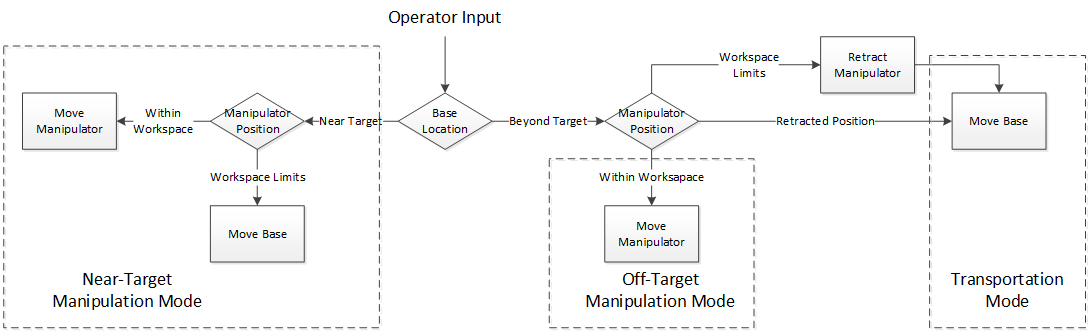
\includegraphics[width=\textwidth]{Drawing24.png}
    \caption{Location-Based Control Algorithm}
    \label{fig:flow}
\end{figure} 

\subsubsection{Transportation Mode}

The transportation mode of the command strategy is used when the operator is driving the base of the MMS. The operator controls the robot using the haptic joystick in world coordinates, using velocity control. The operator can drive the base backward, forwards, left, right, or any combination of these directions by moving the user input device in the direction they want the robot to travel. Since the operator controls the MMS in world coordinates the base will always move relative to the operator's fixed location regardless of its orientation. To rotate the base, the operator uses the buttons located on the Falcon's end-effector. The operator can move the joystick up and down, but it will have no effect on the base motion. In transportation mode, the dead-band is a cylinder that passes through the master's workspace centre and is oriented parallel to the Z axis instead of a sphere centred in the workspace. The velocity of the base is represented by: 
\begin{align}
V_x = C_V\left(J_x\cos\theta - J_y\sin\theta\right)\\
V_y = C_V\left(J_x\sin\theta + J_y\cos\theta\right)
\end{align} 
where $V_x$ and $V_y$ are the base velocities in the $x$ and $y$ directions, $J_x$ and $J_y$ are the joystick positions in the $x$ and $y$ directions, $\theta$ is the base orientation relative to the operator, and $C_V$ is a scaling factor to convert from joystick position to desired base velocity.\\

Due to the design of the drive linkage of the Omnibot's wheels used in this work, there is significant backlash that cannot be predicted. In practice, this means that occasionally the base will lose its desired orientation. To compensate, a yaw control algorithm is implemented such that 
\begin{align}
V_{\theta} = -\theta C_{\theta}
\end{align}
where $C_{\theta}$ is a scaling factor to control the speed of the orientation correction.\\

When driving the MMS in transportation mode, the operator experiences both operation forces and virtual fixtures. The operation forces are to help the operator return the master to the dead-band. When the joystick's end-effector is displaced from the dead-band a centring force is employed to guide the end-effector back into the dead-band. The centring force increases the further away from the dead-band the end-effector gets, and is represented as: 
\begin{align}
 F_i = \begin{cases} 0 & \quad J_i<Db\\ (J_i - M_i)C_G & \quad J_i>Db\\ \end{cases} 
\end{align}
where $F_i$ is the force for axis $i$, $J_i$ is the joystick position in axis $i$, $M_i$ is the haptic force in axis $i$, $C_G$ is the gain, $Db$ is the size of the dead-band, and $i=x,y,z$. When $M_i=0$ only the centring force is felt, additional forces are not added to the overall force displayed, instead the location to which the centring force guides the operator is moved while the location of the dead-band remains unchanged. Using the magnitude of the centring force when no other forces are present, the operator can estimate the velocity of the robot without requiring visual or auditory feedback.\\

The centring force is twofold in purpose: it not only assists the operator in controlling the robot, but it can provide a secondary channel of information to the operator about the robot. In this case, the relationship between the centring force and the robot's velocity is linear so, with experience, the operator is able to estimate the robot's speed not only through a visual cue but tactile as well.\\

The second type of haptic information employed on the haptic master during transportation mode is a forbidden-region virtual fixture. It is used to prevent the operator from colliding with walls or obstacles in its environment. When the operator is within a certain range of an obstacle, they will feel a repelling force when attempting to drive into the obstacle. The force of the virtual fixture is represented by: \begin{align}
M = F_{max}(b/T)C_F
\end{align}
where $0 < b < T$ is the distance past the beginning of the virtual wall the robot has crossed, $T$ is the the thickness of the virtual wall (the region where force is felt but the robot can still move further toward the wall), $F_{max}$ is the maximum force the wall can exert, and $C_F$ is a scaling factor to convert robot distance to joystick force. $M$ is subject to the conditions that the base position $P$ is on the correct side of the wall, within the thickness $T$ of it, and within the defined ranges of the other two axes. To further enforce the collision prevention absolute fixtures are used. Once the robot is within the maximum allowable proximity to the obstacle ($b = T$), it will no longer drive towards it and will ignore any operator commands to do so.\\

\subsubsection{Off-Target Manipulation Mode}

The system enters off-target manipulation mode when the system is more than $D$ distance away from a point of interest. In this manipulation mode the operator controls the velocity of the slave manipulator's end-effector using the master's end-effector similar to the way the base is controlled in transportation mode. Control is performed in world coordinates, such that the operator controls the manipulator relative to their own position regardless of the robot's orientation. Motion is defined as:
\begin{align}
V_i = C_MJ_i
\end{align}
where $J_i$ represents the displacement of the master end-effector from the dead-band, $V_i$ is the slave manipulator's end-effector velocity, and $i=x,y,z$. $C_M$ is used as a scaling factor to increase or decrease the maximum velocity of the manipulator.\\

When controlling the manipulator in off-target manipulation mode the operator will feel two distinct operating forces. The same centring force used in transportation mode is felt during off-target manipulation mode and is felt for any configuration of the manipulator. The centring force will guide the operator's joystick towards the spherical dead-band. When the joystick is within its dead-band, the manipulator does not move. The centring force only centres the joystick, not the manipulator. A second force called the virtual wall is a configuration dependant force only felt in certain positions. The virtual wall exists as a virtual construct that can only be interacted with through the haptic device. Six virtual walls exist within the workspace of the MMS manipulator arm and form a rectangular block represented in Fig. \ref{fig:vwalls}. The location of these walls are chosen such that they enclose a workspace for the manipulator that exists entirely in front of the MMS and no manipulator singularities occur within the boundaries. The walls are given a thickness $T$ and the allowable workspace of the manipulator extends to the outside edge of the virtual walls. When the end-effector of the manipulator is within the inside edge of the walls, no forces additional to the centring force are felt. Once the operator drives the end-effector through the inside edge of the virtual wall they begin to feel the repulsive force of the wall. The virtual wall's repulsive force has the same direction as the centring force, but larger magnitude and is defined just like the base virtual walls:
\begin{align}
M = F_{max}(b/T)C_A
\end{align}
with a different scaling factor $C_A$ but the same conditions. The repulsive force increases in magnitude until it reaches its maximum value at the outer edge of the virtual wall.\\

\begin{figure}[htbp!]
    \centering
    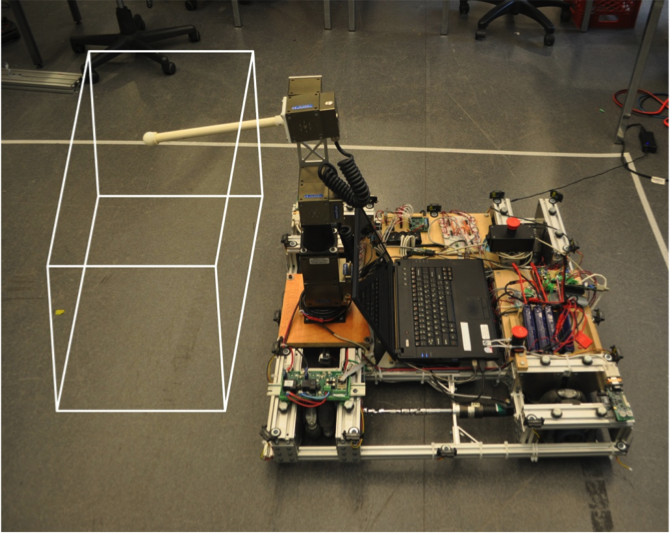
\includegraphics[width=0.7\textwidth]{wallbox.png}
    \caption{Omnibot Manipulator With Virtual Walls Illustrated}
    \label{fig:vwalls}
\end{figure} 

When the manipulator's end-effector reaches the outside edge of the virtual wall, and the operator commands the end-effector to continue moving in a direction outside the wall, the system switches from off-target manipulation mode to transportation mode. The purpose of the virtual wall thickness is to give the operator advance notice that they are about to switch modes and the opportunity to avoid it. When the system enters transportation mode, it will remain in that mode until one of three events occur: a time out, a press of the mode selector button, or the system enters a near-target manipulation mode area. The time out occurs after $t$ seconds of inactivity, indicating that the operator has positioned the base at the desired location and is ready to begin manipulation using the robot arm. If the operator does not wait for the time out and presses the mode selector button, the system returns to off-target manipulation mode immediately. When the system enters a near-target manipulation mode region it automatically switches to near-target manipulation mode.\\

When the system switches from off-target manipulation mode to transportation mode, the manipulator retracts from the point where it breached the outer edge of the virtual wall to a predefined optimal location. The manipulator optimal location was chosen so that the majority of the manipulator's useable workspace was in front of the end-effector, while there was still some room for it to move backwards. Through experimentation, this point was found to be three quarters of the distance from the front virtual wall to the back virtual wall, measured from the front virtual wall.\\

\subsubsection{Near-Target Manipulation Mode}

The system enters near-target manipulation mode when the MMS base is within a near-target manipulation mode region. These regions are circular areas centred around specific points of interest with their radius equal to 80\% the distance from the end-effector to the inside edge of the virtual wall. With the near-target region defined as such, the system will enter near-target manipulation mode only when sufficiently close to the point of interest that the manipulator can interact with it without the base having to move.\\

When controlling the manipulator the operator uses the same technique as in off-target manipulation mode, controlling the manipulator in world coordinates. The centring force, virtual wall location, and virtual wall forces are all identical. The difference between the two manipulation modes is noticed when the manipulator's end-effector reaches the outside edge of the virtual wall. Instead of switching to transportation mode, the system remains in near-target manipulation mode but the operator is able to drive the base. This allows for easy repositioning of the base if the operator is attempting to interact with an object outside the virtual walls, and requires a small movement in the base positioning.\\

When the end-effector reaches the outer limit of the virtual wall and the joystick is not within the dead-band the base will move according to the transportation mode scheme, but the manipulator's end-effector will remain at its location on the edge of the virtual wall. The operator will continue to feel the centring force and virtual wall force while driving the base. As long as the operator commands the manipulator to move outside the virtual wall while it's at the edge, the base will move. If at any time the operator commands the end-effector away from the edge of the virtual wall, even while driving the base, the MMS base will cease movement and the manipulator will move. The system will only enter this pseudo-transportation mode while the end-effector is at the virtual wall's outer edge and the haptic joystick is outside the dead-band in the direction of the virtual wall and will only remain in that mode while these conditions are met. When the operator moves the master to the dead-band or out of the dead-band in the direction opposite to the virtual wall the system returns to near-target manipulation mode.\\

If the operator intends to switch to transportation mode, they will have to use near-target manipulation mode to drive the base outside the near-target manipulation mode region. Outside the near-target region the system enters off-target manipulation mode. At the instant the MMS leaves the region, the state of the system is such that the end-effector is at the outside limit of the virtual wall, and the haptic master is outside the dead-band in the direction of the virtual wall. In this state during off-target manipulation mode, the end-effector retracts to its optimal position and the MMS enters and remains in transportation mode. To the operator, as the MMS drives out of a near-target region, they will notice the arm retract to its optimal position as the system switches from pseudo-transportation mode to the regular transportation mode. During the mode switch the operator is not required to adjust their actions, it occurs entirely autonomously and the operator need only focus on continuing to drive the base of the MMS.\\


\section{Test Platform}
\label{sec:back}
To develop a new command strategy for controlling a MMS via a haptic input device, a suitable test bed was required. There are three main elements to the required test bed: the base and the arm form the MMS and the haptic joystick is the user input device. In this work, the Omnibot MMS was used with a Novint Falcon haptic joystick.\\

\subsection{Omnibot MMS}
The Omnibot MMS consists of two parts: the arm and the base as shown in Figure \ref{fig:vwalls}. The arm is a 3-DOF manipulator made from Schunk Powercube rotary modules. It is capable of positioning anywhere within the predefined rectangular block-shaped workspace without any singularities. It is mounted on the Omnibot base so the majority of its workspace is in front of the base.\\

The base is an omnidirectional platform capable of driving in any direction on the surface it sits on, while simultaneously rotating around an axis perpendicular to that plane. It achieves holonomic manoeuvring capabilities through the use of omni-wheels. Four omni-wheels are located orthogonally on the Omnibot. Each omni-wheel has a passive and active direction. The passive direction is along the active wheel's axis of rotation, meaning it can slide freely perpendicular to the direction it is being driven. A detailed study of the Omnibot's design can be found in \cite{bemis}. By having two wheels in one axis of the robot, and two in a perpendicular axis, omnidirectional motion is achieved through varying the velocities of the four wheels on the Omnibot. The omnidirectional motion of the base allows for the command strategy to utilize motions that are not possible for a non-holonomic MMS. By increasing the manoeuvrability of the MMS, the command strategy for the system can be less restrictive and easier to use by both inexperienced and experienced operators.\\
 
The Omnibot MMS is fitted with a number of on-board sensor and communication devices. The Omnibot uses the Robot Operating System (ROS) to facilitate the operation and communication of the various software programs that run on the main workstation. ROS is a software framework for robot software development using multiple software \textit{Nodes} that communicate by \textit{Posting} and \textit{Subscribing} to \textit{Topics}. Initially developed at Stanford Artificial Intelligence Library and expanded by Willow Garage, current stewardship resides with the Open Source Robotics Foundation (www.ros.org).\\

The original Omnibot localization system used Cricket ultrasonic range finders to locate its position within the robot's workspace. Using a configuration with two robot mounted beacons and a fixed array of listeners the Omnibot was able to localize its position and orientation, but suffered from poor accuracy. Details of the Cricket localization system can be found in \cite{sasha}.\\

With recent updates to the Omnibot localization system, the Crickets have been replaced with an OptiTrack motion capture system. This is a much needed improvement to the Omnibot since the Crickets suffer from significantly poor accuracy. Using the motion capture system the positional accuracy has been improved from 5-10 cm accuracy to sub-millimeter levels. While the use of a Kalman filter to combine the Cricket and motion capture data would lead to even better accuracy, the motion capture system alone is sufficient for this application and reduces the overall complexity of the localization as well as computational cost.\\

%Figure \ref{fig:flowchart} shows an overview of the entire Omnibot MMS. The majority of the computational work is done on the remote desktop. Running ROS, the remote desktop uses five ROS nodes to perform its given tasks. The features of the command strategy are programmed within the Fixtures node, with the four other nodes on the remote desktop facilitating communication with the joystick, motion capture device, Omnibot, and the user (for activating/deactivating the virtual fixtures and datalogging feature). The cameras for the motion capture system connect to the Optitrack computer, which uses Optitrack's Tracking Tools software to track objects within the work cell and broadcast their positions using NATNet protocols. The Mocap node on the remote desktop reads the motion capture broadcast data and publishes the Omnibot MMS pose and target data through ROS to be read by the Fixtures node. The Joystick node uses the Falcon Application Programming Interface (API) to communicate through USB to the Falcon joystick. The Joystick node receives force commands from Fixtures and sends the joystick position back. The Datalogger node provides a command line interface to the system, allowing the operator to enable/disable the virtual fixtures as well as record the experimental data. The Talker node uses TCP IP socket communication to send the movement commands it receives through ROS from the Fixtures node. The Talker node also receives the joint configuration of the manipulator so it can calculate the manipulator's local pose using forward kinematics. The manipulator's pose in local coordinates are received by the Fixtures node through ROS, and the manipulator and base's position in global coordinates are sent to the Fixtures node via the Optitrack computer and Mocap node.\\


The on-board computer on the Omnibot MMS is responsible for receiving motion commands from the Talker node on the remote desktop and executing the desired actions. The Powercube rotary modules that form the manipulator arm are controlled via a USB-CAN interface connected to the on-board computer. Using the Powercube Application Program Interface (API) and the manipulator's inverse Jacobian matrix the desired end-effector velocity is converted to a set of joint rates. The integrated encoders on the rotary modules are read through the CAN bus and sent back to the remote desktop.\\

Using serial communication, an Arduino MEGA microcontroller responsible for motor control is sent the desired wheel velocities through USB. Using two dual motor drivers the power of each motor is controlled via Pulse Width Modulation (PWM). Each motor's encoder is constantly read using a 16-bit encoder counter and polled intermittently for the latest data by the Arduino. The Proportional-Integral-Derivative (PID) control of the motor is done by the Arduino microcontroller.\\

\subsubsection{PID Control}

There is a significant amount of backlash in the motor linkage on the Omnibot. This, coupled with the high gearing ratio of the motors, makes accurate control of the wheels a non trivial matter. To overcome the physical limitations of the system, a closed-loop control system is employed using PID control. The correlation between motor speed $S$ and PWM duty cycle $D$ is:
\begin{align}
D = \alpha e ^{S\beta}
\end{align}
where the motor constants $\alpha$ and $\beta$ are found in Table \ref{tab:pid}. Once the relation between power and speed was determined experimentally for each motor a PID control system was implemented using the control gain values $K_P = 3$, $K_I = 0.002$, and $K_D = 1$.\\


\begin{table}
\centering
\caption{Motor Parameters}
\begin{tabular}{ l | c | c | }
\cline{2-3}
  & $\alpha$-parameter & $\beta$-parameter \\ \cline{2-3}
Motor 1 & 33.988 & 1.655 \\ \cline{2-3}
Motor 2 & 33.007 & 1.652 \\ \cline{2-3}
Motor 3 & 34.295 & 1.650 \\ \cline{2-3}
Motor 4 & 31.910 & 1.700 \\ \cline{2-3}
\end{tabular}
\label{tab:pid}
\end{table}

\subsection{User Input Device}

%The Omnibot can be controlled by the 3-DOF planar joystick shown in Fig. \ref{fig:joystick}. The joystick has two linear DOF that allow the operator to drive in any direction along the plane the Omnibot is on. A rotational DOF allows the operator to twist the joystick in order to command the Omnibot to rotate around its center. With the addition of the manipulator, making the Omnibot in to the Omnibot MMS, a different user input device was required with three linear DOF to control the manipulator. Early versions of the Omnibot MMS required two user input devices for the operator to control both the base and arm of the MMS and the user was required to control them independently.\\

The user input device selected to command the manipulator of the Omnibot MMS is the ``Falcon'' made by Novint Technologies. The Falcon is a cost effective impedance type haptic joystick capable of using 3-dimensional (3D) positioning data as an input and producing forces along those 3-dimensions as outputs. The positional input has an accuracy of 157 dpcm (400 dpi) across its 10 cm$\times$10 cm$\times$10 cm ($4 ''\times4 ''\times4 ''$) workspace. The force displayed is a minimum of 8.9 N (2 lbs) within its workspace. The Falcon also has four buttons located on its end-effector. An image of the Falcon is shown in Fig. \ref{fig:falcon}.

\begin{figure}[htbp!]
    \centering
    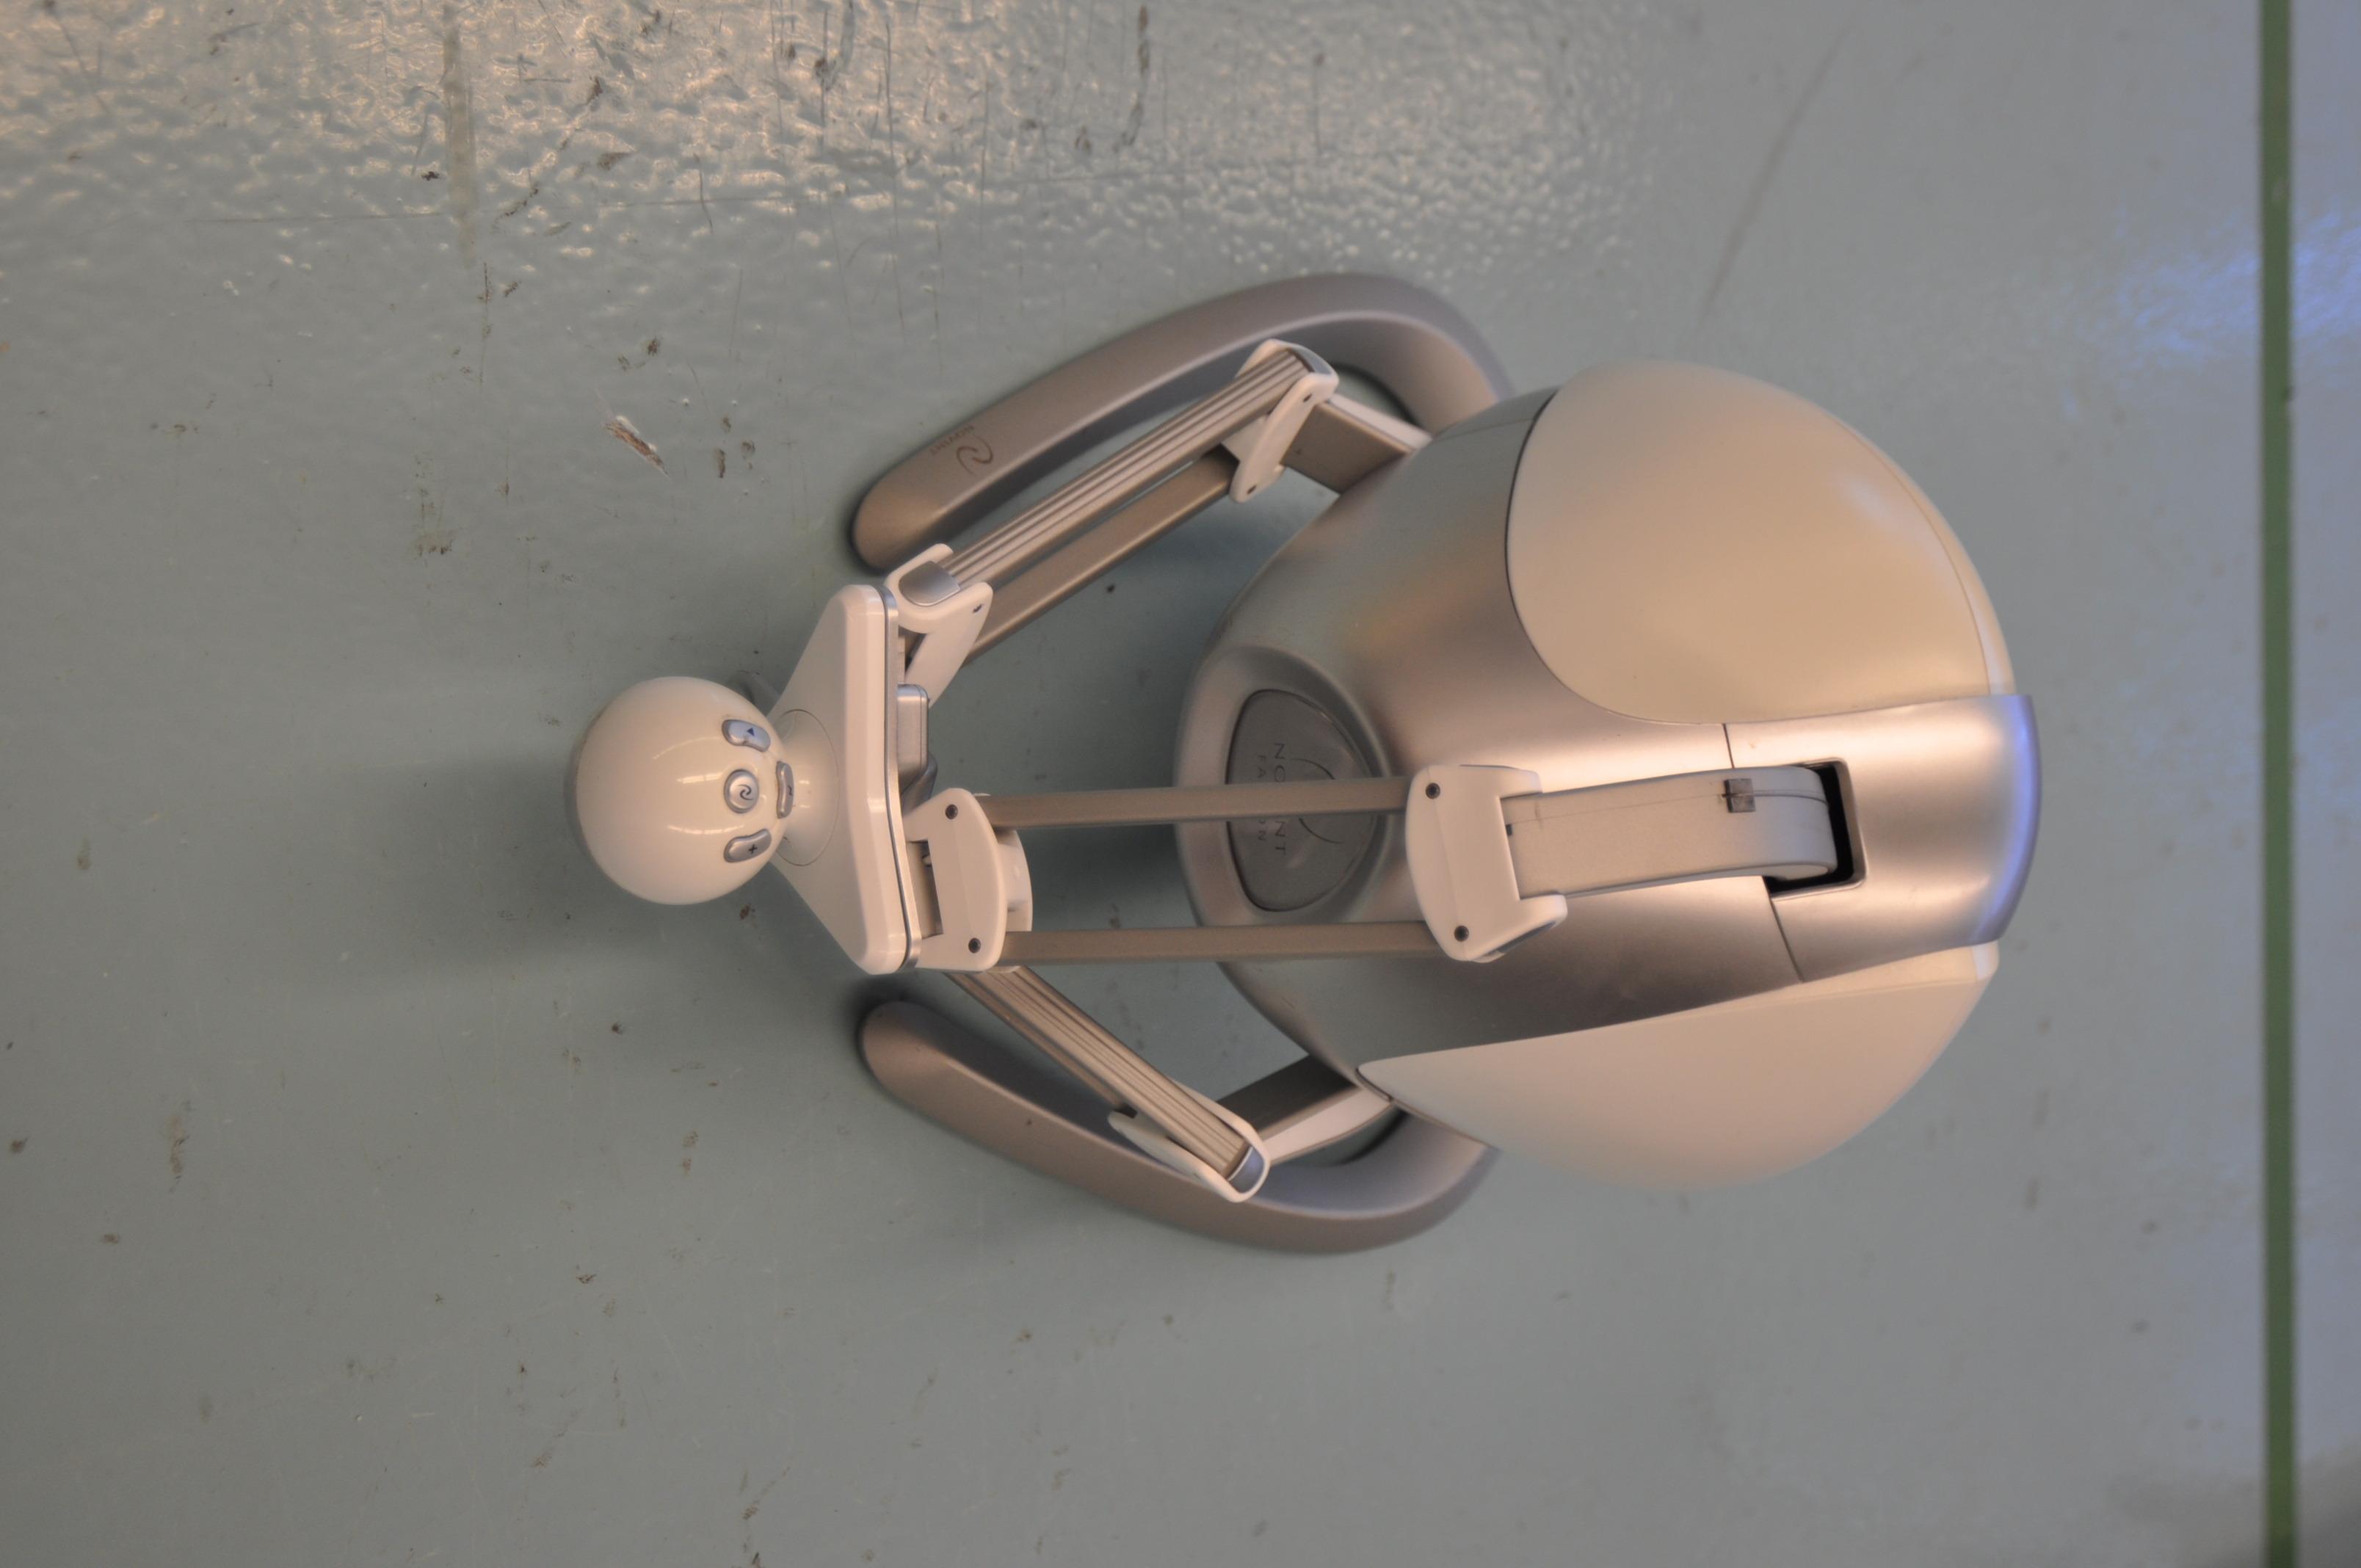
\includegraphics[width=0.4\textwidth, angle = 90]{DSC_0228.jpg}
    \caption{Falcon Joystick}
    \label{fig:falcon}
\end{figure} 

The command strategy was developed to be used with a 3-DOF haptic joystick. The operator must be able to position the MMS end-effector in 3-dimensions, position the MMS base ``Omnibot'' in two dimensions, and orient the Omnibot in one dimension. While only 3-DOF is required for both positioning and orientation of the MMS base, representing a rotational DOF with a positional DOF would be very confusing to the operator. Since most haptic devices come in 3-DOF or 6-DOF varieties, the Falcon was chosen in part due to its abilities to simulate a rotational DOF using the buttons located on the end-effector. To simulate a rotational DOF, the left and right buttons on the end-effector simulate a counter-clockwise and clockwise rotation, respectively. Though the rotational DOF only have a unit response, the fixed rotation rate used did not hinder the operator's ability to orient the Omnibot MMS as required. In later testing, orientation became less significant as the test-scenario did not require the operator to change orientation of the base.\\

\section{Experimentation Using the Command Strategy}
\label{sec:results}
To test the effectiveness of the command strategy, a typical pick-and-place scenario was designed. This scenario requires the operator to utilize the various features of the command strategy, while minimizing the effect of some of the Omnibot MMS design limitations. Mainly, the lack of a gripper tool on the end-effector, and the difficulty in controlling the rotational DOF for the Omnibot base. To overcome the limitations, the pick-and-place task is simulated using the targets shown inset in Fig. \ref{fig:setup}. The targets can be knocked over using the end-effector of the manipulator. This action requires the operator to perform very similar motions to a pick-and-place task, and tests their ability to accurately control the manipulator in small motions. There are two pick-and-place stations to be completed in the first evaluation scenario, and driving between the two stations tests the operator's ability to accurately control the MMS base.\\

Since the joystick only rotates the base at a fixed rate, the two pick-and-place stations are oriented the same way so the operator does not need to rotate the Omnibot when completing the test scenario. Though no change in orientation is required, the operator's skill in driving the Omnibot is still adequately tested as they navigate through the experimental set-up. It is the authors' belief that the lack of orientation change throughout the experiment does not affect the evaluation of the operators' performance.\\


\subsection{Experimental Set-Up}

The first experimental set-up is shown in Fig. \ref{fig:setuptest}. In the test scenario, the operator is required to begin with the Omnibot MMS located at its start location shown in Fig. \ref{fig:setuptest}. From the start location, the operator must drive the MMS to the first pick-and-place station. At the first station they simulate the pick-and-place task by knocking over the two targets. Upon completion of the task, the operator must navigate around the dividing wall to the second pick-and-place station and perform the second pick-and-place task by knocking over the two targets at that location. After the final task is completed, the operator must drive the robot back to its start position to complete the scenario. The operator uses both line of sight and haptic feedback to perform the test. Figures \ref{fig:setuptest} and \ref{fig:setup} show the test areas from the operator's perspective.\\

\begin{figure}[htbp!]
    \centering
    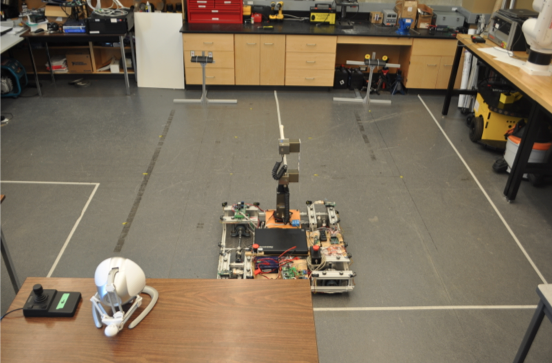
\includegraphics[width=\textwidth]{test1.png}
    \caption{Photo of Preliminary Testing Configuration for Test Scenario}
    \label{fig:setuptest}
\end{figure} 

To compare the novel single input device command strategy with the traditional two input device command strategy, the test runs for the two command strategies were interleaved. The operator did a single run using the first command strategy, followed by another run with the second command strategy. The pattern is followed until sufficient data was collected. The old command strategy required the operator to use two joysticks, one joystick controls the Omnibot base, and the second joystick controls the MMS arm. When using the new command strategy, only a single joystick was used along with the virtual fixtures and operational forces. There were no virtual fixtures in the old command strategy, and the only operation forces felt are the centring forces. The virtual wall still exists but is not felt, and when the end-effector reaches the virtual wall it simply stops moving.\\

\subsection{Initial Experimental Results}

Four novice users were chosen to evaluate the command strategy, and one expert user was used as a baseline for comparison. The novice users had no previous experience with the Omnibot MMS or the command strategy. The expert user had a significant amount of experience with the Omnibot MMS and both the new and old command strategies. The purpose of having an expert user was to offer a comparison of how well the novice operators performed versus an experienced operator. Though performance will vary from user to user, it is valuable to have an idea of how well the system performs under experienced operator control.\\
\begin{table}[htbp!]
\caption{Averaged Timing Results from Preliminary Testing}
\noindent\makebox[\columnwidth]{
\resizebox{\textwidth}{!}{
    \begin{tabular}{|r|r|r|r|r|r|r|r|}
    \hline
         & \multicolumn{4}{c|}{Single Joystick} & \multicolumn{3}{c|}{Dual Joystick} \\
    \hline
    		& Completion Time (s) & Adjusted Completion Time (s) & Base Travel Distance (m) & Average Base Speed (m/s)& Completion Time (s) & Base Travel Distance (m) & Average Base Speed (m/s) \\
    \hline
    User 1 & 106.6 & 94.7 & 15.9 & 0.36 & 91.3 & 18.3 & 0.5 \\
    \hline
    User 2 & 84.8 & 60.6 & 19.4 & 0.38 & 107.6 & 18.8 & 0.71 \\
    \hline
    User 3 & 101.1 & 81.5 & 17.2 & 0.32 & 86.7 & 17.3 & 0.51 \\
    \hline
    User 4 & 86.2 & 78.2 & 16.0  & 0.37 & 101.8 & 18.9 & 0.46 \\
    \hline
    Average & 94.7 & 78.8 & 17.1 & 0.36 & 96.9 & 18.3 & 0.55 \\
    \hline
    Expert User & 58.8 & 71.6 & 15.2 & 0.44 & 106.4 & 19.6 & 0.32 \\
    \hline
    \end{tabular}
}
}
\label{tab:results}
\end{table}

Table \ref{tab:results} presents the initial test results. Upon first inspection of the results there was barely a noticeable improvement in completion time when using the single joystick command strategy. When the additional information was analysed, it was noted that the operators were able to drive the base much faster using the dual joystick command strategy. There are two explanations for this, the first being simply that the dual joysticks had a slightly higher maximum velocity. The second reason for the slower average speed is due to the localization accuracy and the virtual fixture friction property explained below. An adjusted completion time for the single joystick command strategy was computed where the completion time was calculated based on the velocity of the dual joystick command strategy over the distance travelled in the single joystick command strategy for each operator. The adjusted completion time for the single joystick command strategy yielded an 18\% improvement over the dual joystick command strategy. The expert user was able to complete the task using the single joystick command strategy 25\% faster than the novice users' adjusted completion time, and 38\% faster than their original completion time.\\

The experimental data from the novice users was used to estimate a learning curve. This was done by plotting each operator's completion time for both command strategies, and using a linear line of best fit. As shown in Fig. \ref{fig:curves}, most of the users' learning curves were steeper with the single joystick command strategy. With the learning curves presented in Fig. \ref{fig:curves}, one would assume that the novices' skill using the new command strategy will continue to increase and reach a level equal to the expert operator, while their skill with two joysticks has already neared its maximum potential.\\

When asked which command strategy each operator preferred, all test subjects agreed that the single joystick command strategy was easier and more intuitive to use. It was noted that even though the operators were allowed to use both hands when using both joysticks, they still only used one joystick at a time because it was ``difficult'' and ``stressful'' to attempt to control both manipulator and base simultaneously.\\

The one complaint the novice operators had against the single joystick command strategy was about the virtual fixture friction. While this fixture did prevent the Omnibot MMS from colliding with any walls (represented as taped markings on the floor) the system would often assume the MMS was closer to a wall than it actually was, making it difficult for the operator to navigate through a narrow passage. Since the friction of the virtual fixture was infinite, simply touching it would make moving the robot impossible. The reason for this type of error was due to the accuracy of the Cricket localization system, where it would incorrectly estimate the current position of the MMS. While the operator may still have room to drive in the direction they commanded without a collision, the localization system would assume there was no room to drive in that direction, and the forbidden region virtual fixture would prevent motion. Operators would occasionally get the MMS temporarily ``stuck'' when driving close to a wall, and increase the overall average completion time for the single joystick command strategy making it less efficient than it would be under ideal conditions. Since the forbidden region virtual fixtures were not present in the two joystick command strategy, its average completion time was not affected. To improve localization accuracy and prevent future problems surrounding this issue, the Cricket localization system was replaced by a much more accurate OptiTrack motion capture localization system.\\

\begin{figure}[h]
\begin{center}$
\begin{array}{cc}
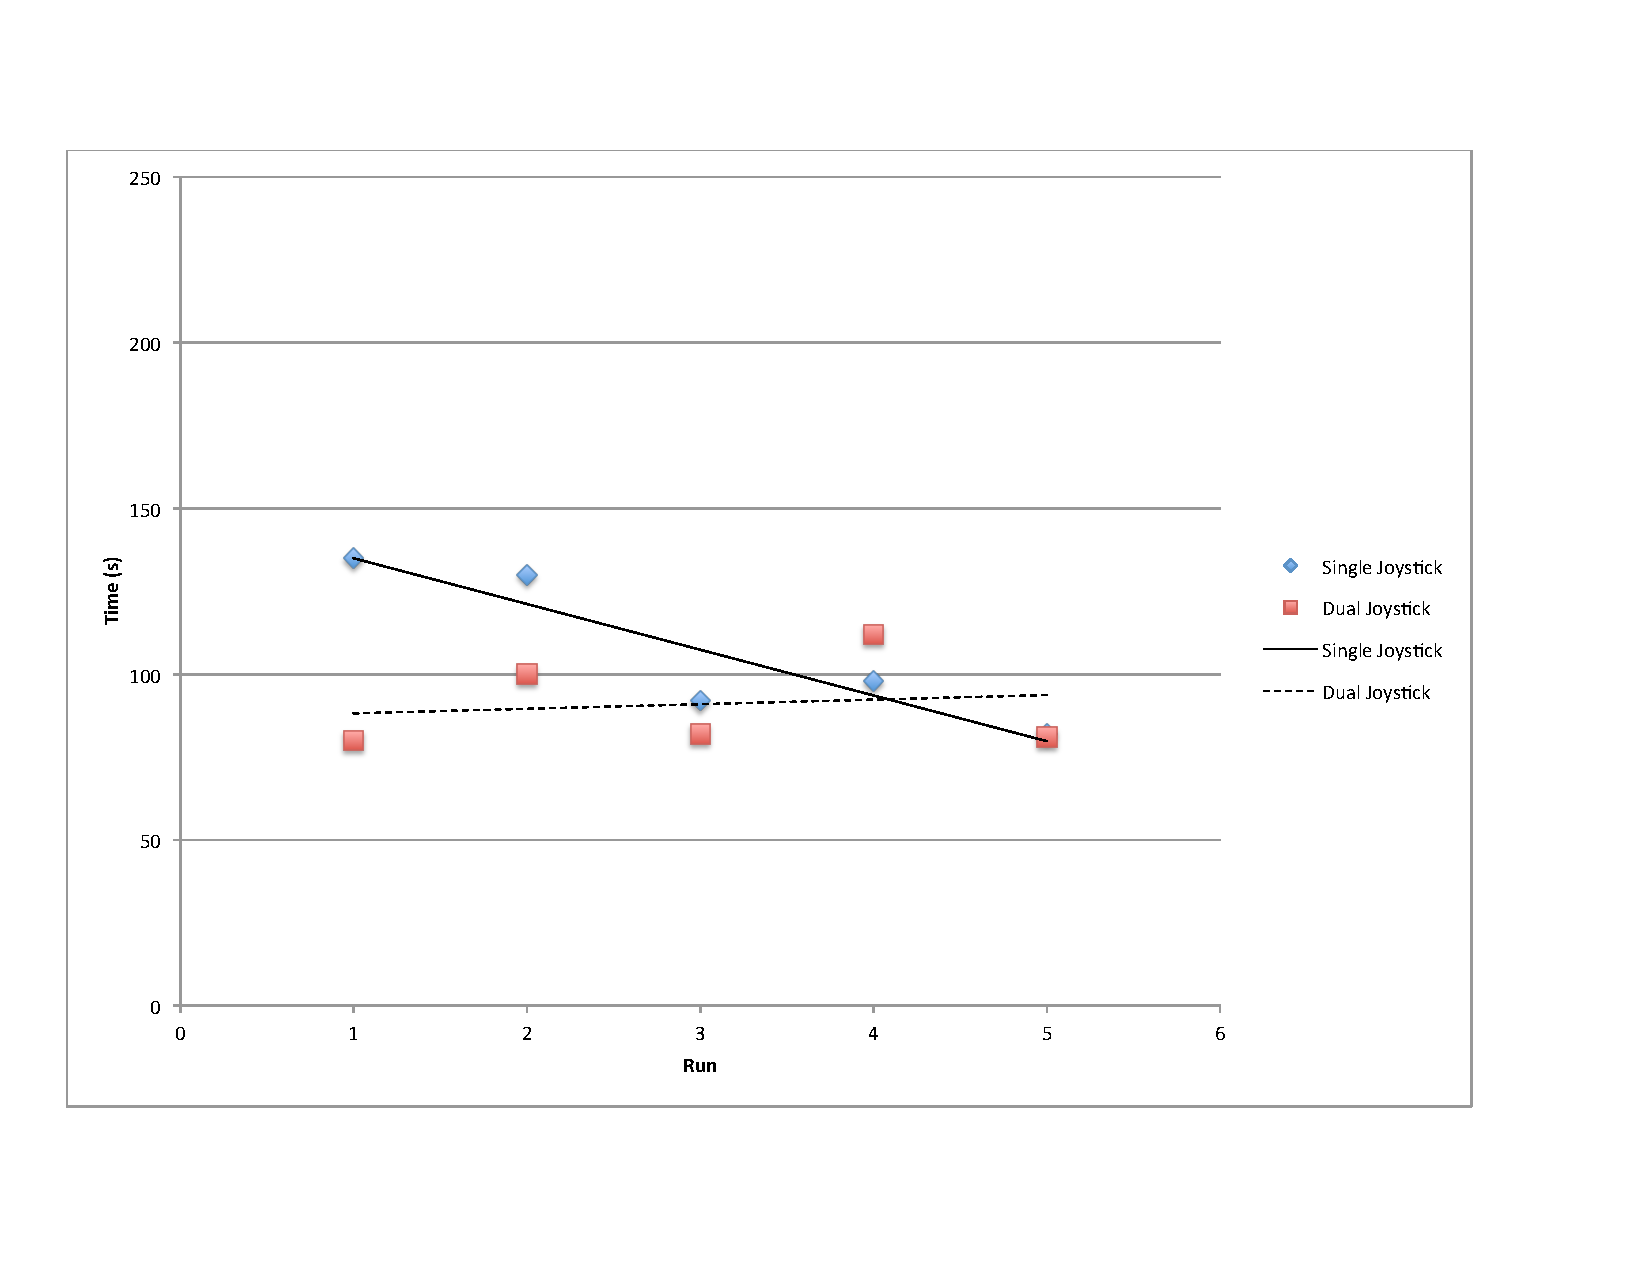
\includegraphics[trim=1.5cm 2.5cm 1.5cm 2.5cm, width=0.5\textwidth]{c1.pdf} &
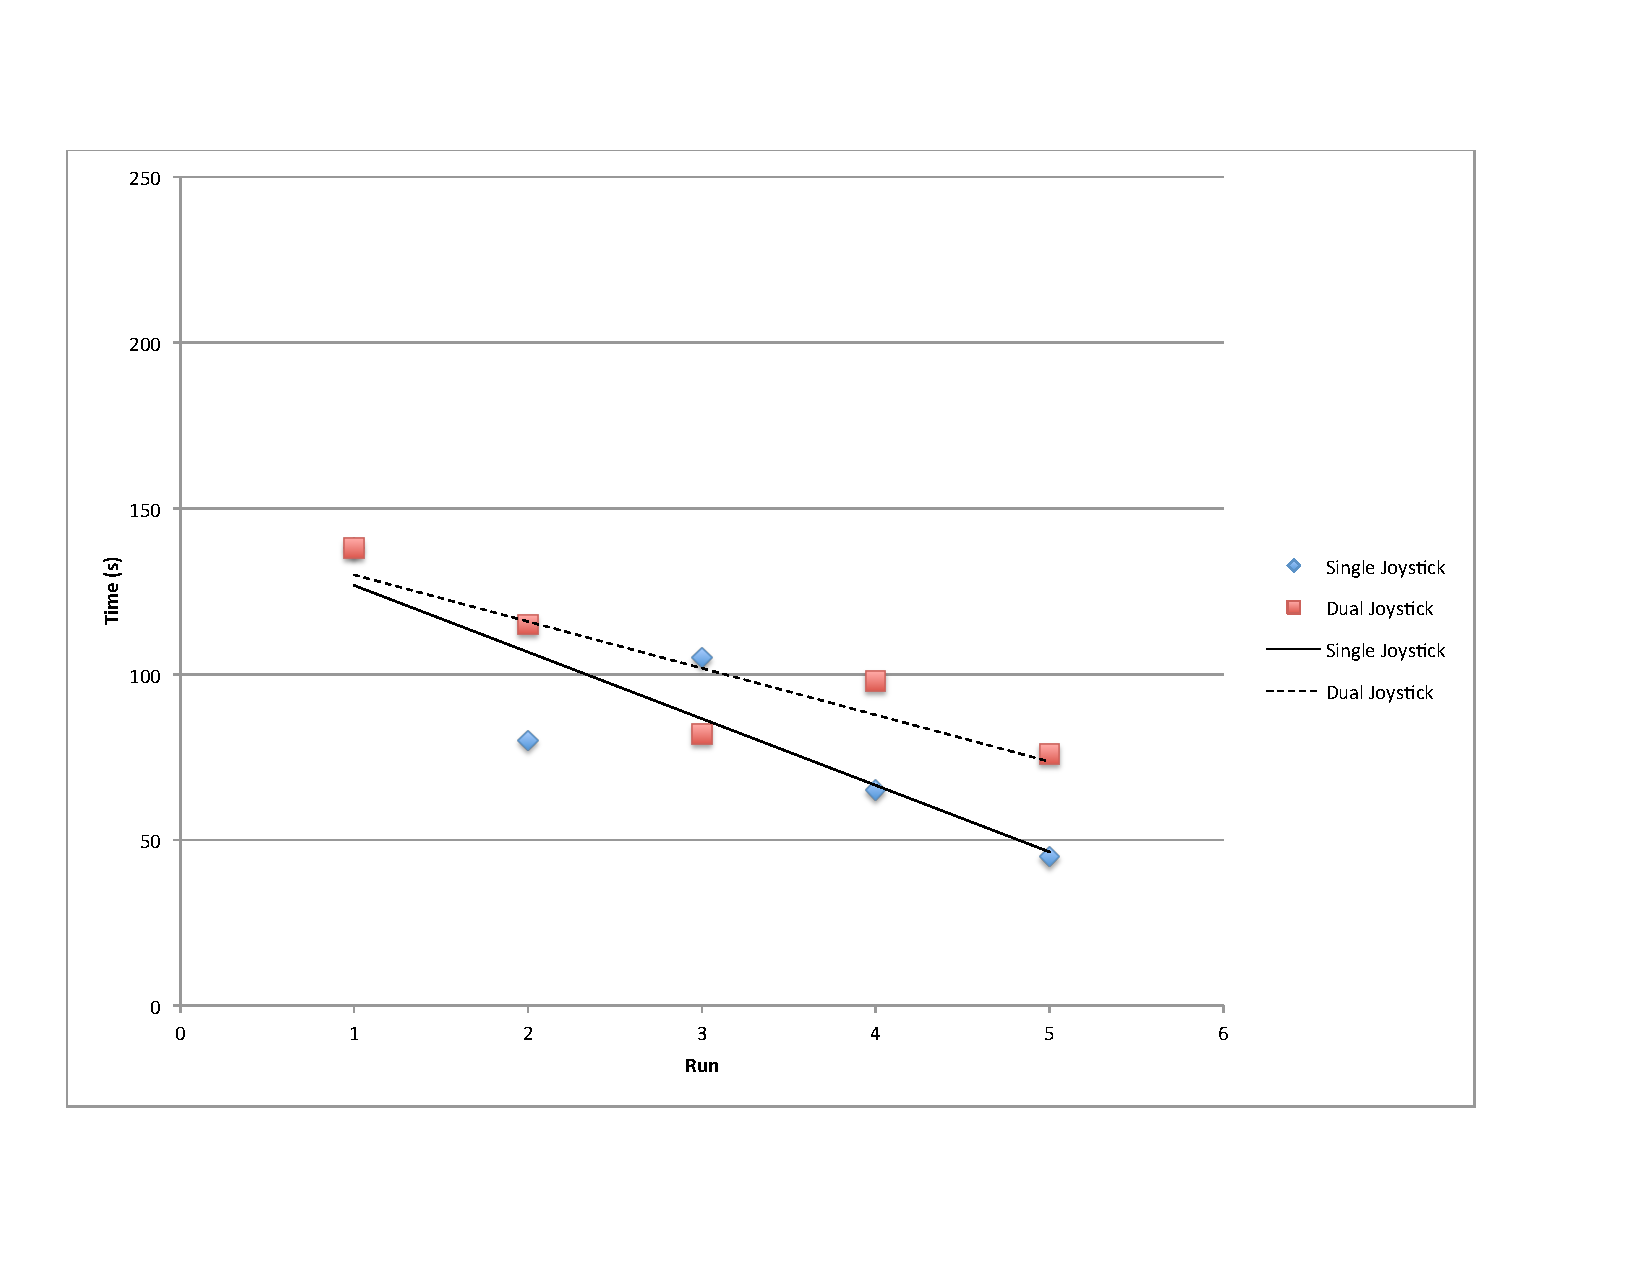
\includegraphics[trim=1.5cm 2.5cm 1.5cm 2.5cm, width=0.5\textwidth]{c2.pdf} \\ 
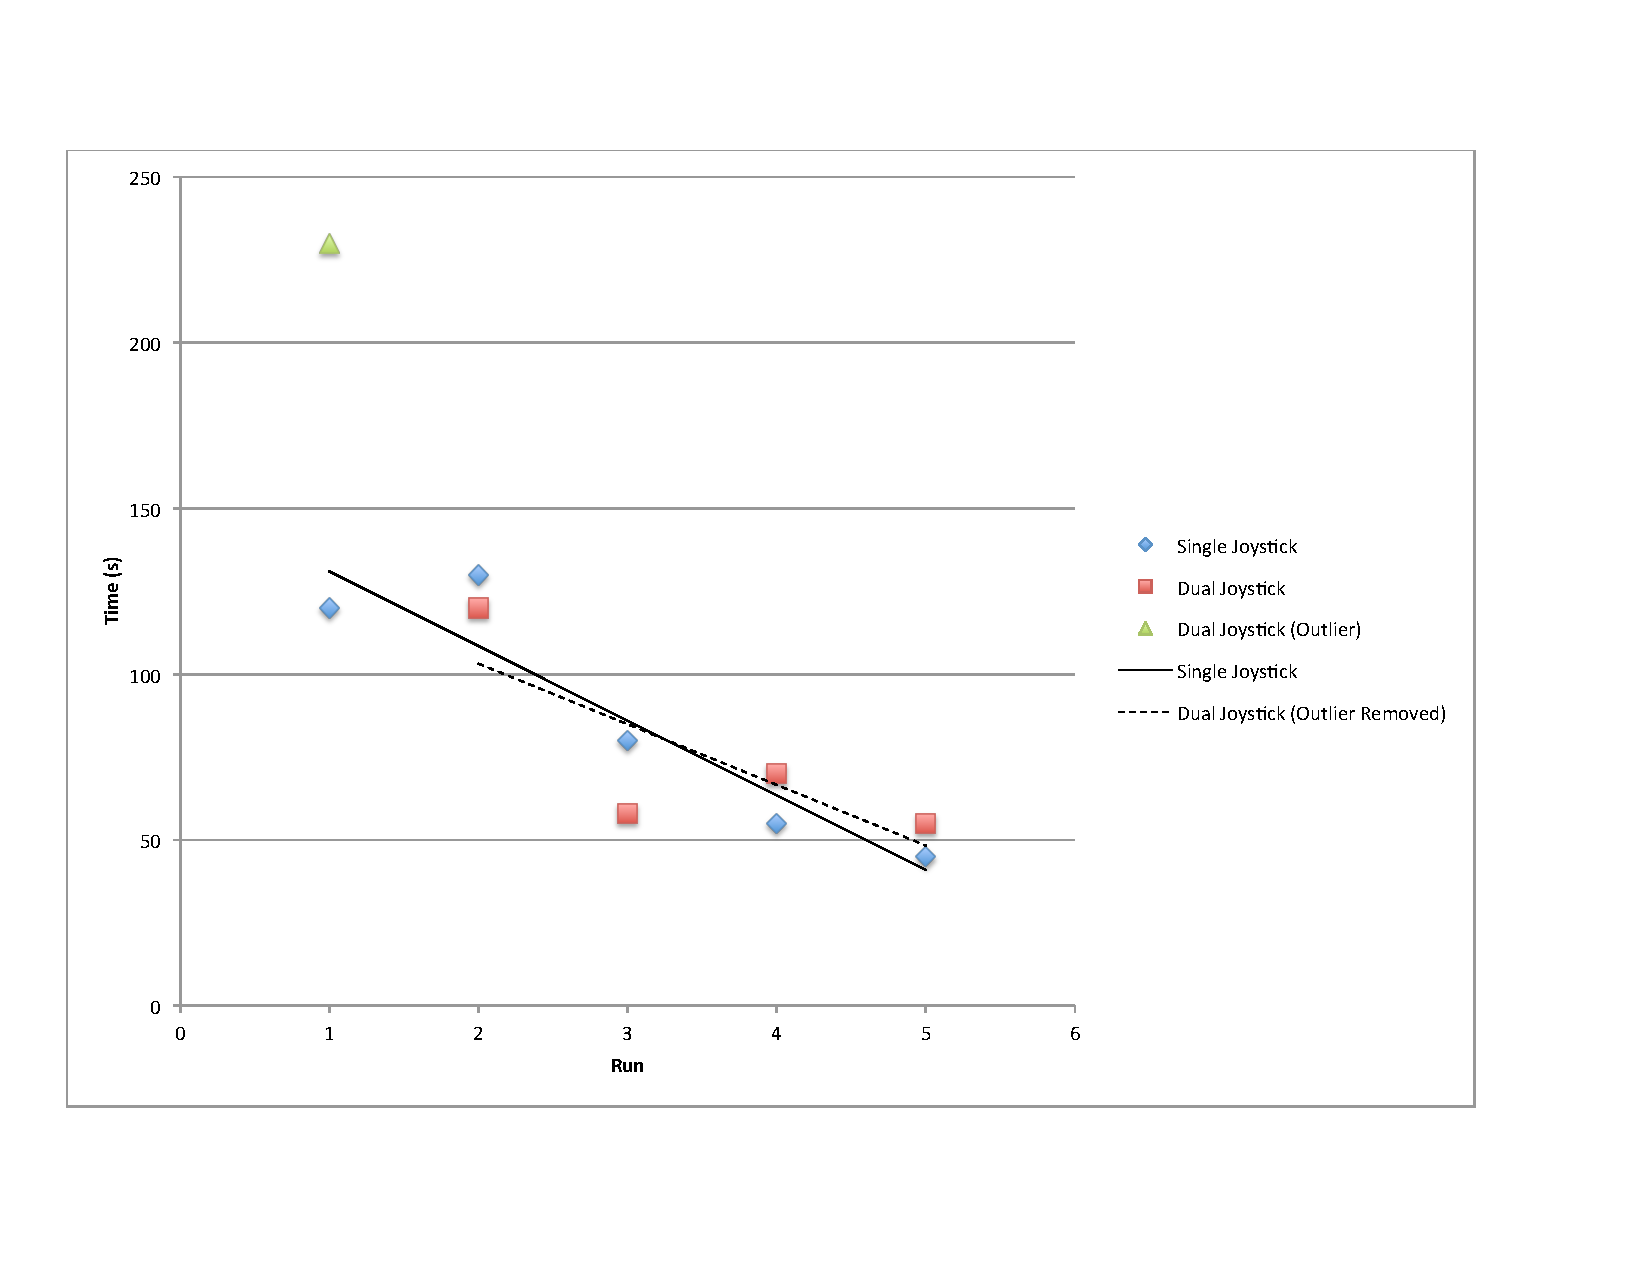
\includegraphics[trim=1.5cm 2.5cm 1.5cm 2.5cm, width=0.5\textwidth]{c3.pdf} &
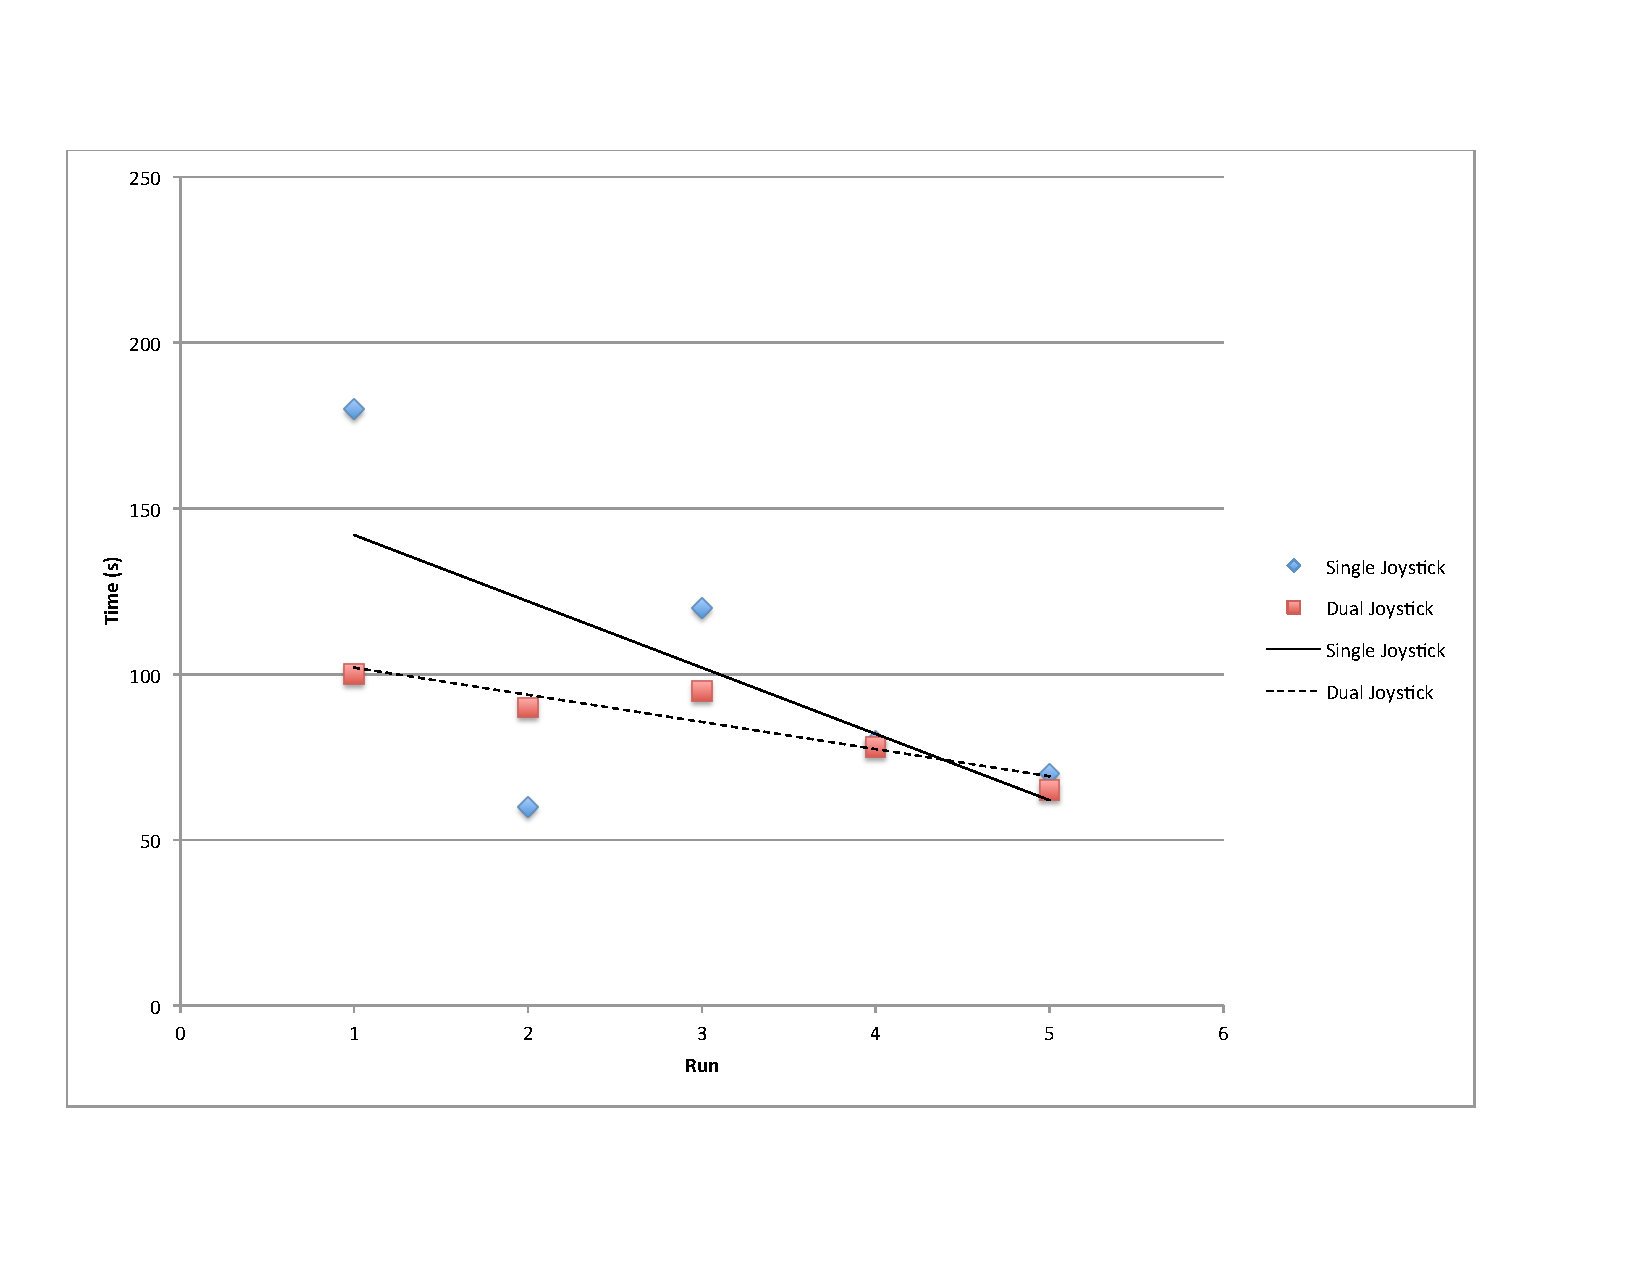
\includegraphics[trim=1.5cm 2.5cm 1.5cm 2.5cm, width=0.5\textwidth]{c4.pdf}
\end{array}$
\end{center}
    \caption{Learning curves for multiple novice test subjects}
    \label{fig:curves}
\end{figure}






\subsection{Refining the Command Strategy}

After the initial round of testing, the command strategy was refined and improved. Since it was shown that the operators were more effective when using a single joystick, it became pertinent to determine the effectiveness of the virtual fixtures. Three important changes were made to the system affecting the accuracy, control, and functionality.

\subsubsection{Accuracy}

The accuracy of the system was greatly improved between the first and second rounds of testing. The ultrasonic localization system based on Crickets was replaced with the OptiTrack motion capture system. This change improved the Omnibot MMS position estimates by two orders of magnitude, from 5-10 cm accuracy to less than a millimeter. Since the positioning accuracy was greatly improved, virtual fixtures based around the pick-and-place targets themselves were now possible.\\

\subsubsection{Control}

The command strategy was altered as well. In the first round of testing, a near-target manipulation mode and off-target manipulation mode was used. While off-target manipulation mode is useful when the operator expects the targets of interest not to be stationary, it is not useful in a scenario where the targets are fixed. For the second round of testing, off-target manipulation mode was removed having the system enter transportation mode any time it was sufficiently far away from a point of interest.\\

\subsubsection{Functionality}

The functionality of some virtual fixtures was changed as well. The friction aspect of the forbidden region virtual fixtures was removed, allowing the users to slide along a wall, rather than stop whenever they touched one. The frictionless virtual fixtures still prevented any motion towards a wall when at its limit, but would allow motion parallel to the fixture.\\

\subsection{Final Experimental Results}

With the above changes implemented, a second experimental scenario was created to test the effectiveness of the virtual fixtures using the refined command strategy. The robot environment was set up as shown in Fig. \ref{fig:setup}, with a single point of interest. Similar to the first experiment, the operator was required to start at the location shown, navigate to the point of interest, perform a manipulation task, and return to their starting point. Though visually enhanced in Fig. \ref{fig:setup}, the walls are represented to the operator as marked lines on the floor. The testing methodology consisted of the operator performing one run without using virtual fixtures, followed by a run using the virtual fixtures.\\

\begin{figure}[htbp!]
    \centering
    \includegraphics[width=\textwidth]{inset2.png}
    \caption{Photo of Experimental Configuration for Test Scenario Taken from the Operator's Perspective with Targets Inset}
    \label{fig:setup}
\end{figure} 

The difficulty of demonstrating the effectiveness of this command strategy is that most test criteria are centred around a specific task, whereas this command strategy must be versatile enough not to need modification for most tasks, and easily changed enough to allow for performing specific tasks. The experiment set-up for this research requires the operator to perform the two-main tasks that a mobile-manipulator system can do: transportation and manipulation. The transportation task was very similar to a real-world application where there are obstacles that an operator must navigate around. The manipulation task was very rudimentary, but sufficiently tested the operator's control of the manipulator by requiring both accuracy and control. The robot end-effector can be modified to attach a specific tool, or designed to hold a variety of interchangeable tools. Ten novice operators were used in the testing of the final command strategy with the timing results presented in Table \ref{tab:results2} and navigation results in Table \ref{tab:results3}.\\


\begin{table}[htbp!]
\caption{Averaged Timing Results from Testing (in seconds)}
\noindent\makebox[\columnwidth]{
\resizebox{0.5\textwidth}{!}{
    \begin{tabular}{rrr}
    \toprule
          & Without Virtual Fixtures & With Virtual Fixtures \\
    \midrule
    User 1 & 74.7 & 52.9 \\
    User 2 & 87.6 & 83.2 \\
    User 3 & 69.0 & 69.6 \\
    User 4 & 66.7 & 52.5 \\
    User 5 & 58.7 & 55.2 \\
    User 6 & 73.3 & 65.9 \\
    User 7 & 57.4 & 46.9 \\
    User 8 & 94.1 & 78.9 \\
    User 9 & 119.7 & 92.5 \\
    User 10 & 169.2 & 107.8 \\
    Average & 87.0 & 70.5 \\
    \bottomrule
    \end{tabular}
}
}
\label{tab:results2}
\end{table}

\begin{table}[htbp!]
\caption{Total Collision Results from Testing}
\noindent\makebox[\columnwidth]{
\resizebox{0.5\textwidth}{!}{
    \begin{tabular}{rrr}
    \toprule
          & Without Virtual Fixtures & With Virtual Fixtures \\
    \midrule
    Collisions & 11 & 5 \\
    Close Calls & 18 & 11 \\
    \bottomrule
    \end{tabular}
}
}
\label{tab:results3}
\end{table}

%\begin{table}[htbp!]
%\caption{Percent Improvement and Completion Time}
%\noindent\makebox[\columnwidth]{
%\resizebox{0.5\textwidth}{!}{
%    \begin{tabular}{rrr}
%    \toprule
%          & Completion Time & Percent Improvement \\
%    \midrule
%    User 1 & 57.4326& 18.3\\
%    User 2 & 58.7717& 6.1\\
%    User 3 & 66.7742& 21.3\\
%    User 4 &69.0623 & -0.9\\
%    User 5 & 73.3809& 10.1\\
%    User 6 &74.7379 & 29.2\\
%    User 7 & 87.6695& 5.0\\
%    User 8 & 94.1344& 16.1\\
%    User 9 &119.768 & 22.8\\
%    User 10 &169.217 & 36.3\\
%    Average & & 70.5768 \\
%    \bottomrule
%    \end{tabular}
%}
%}
%\label{tab:results2}
%\end{table}

\begin{figure}[htbp!]
    \centering
    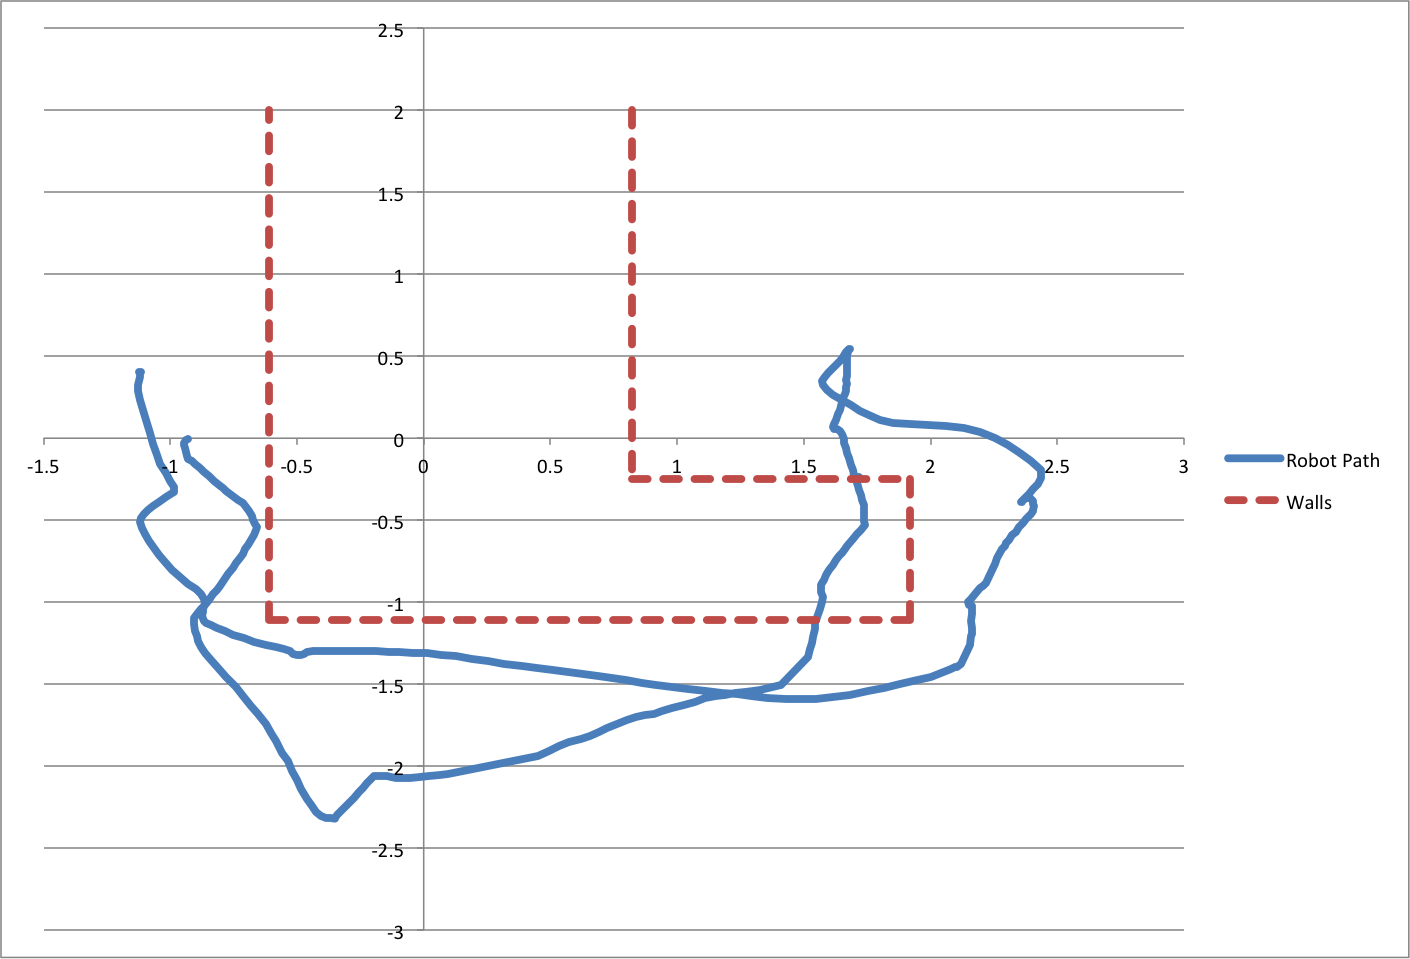
\includegraphics[width=0.8\textwidth]{collisions.png}
    \caption{Example of a Test Run Without Virtual Fixtures}
    \label{fig:collisions}
\end{figure} 

\begin{figure}[htbp!]
    \centering
    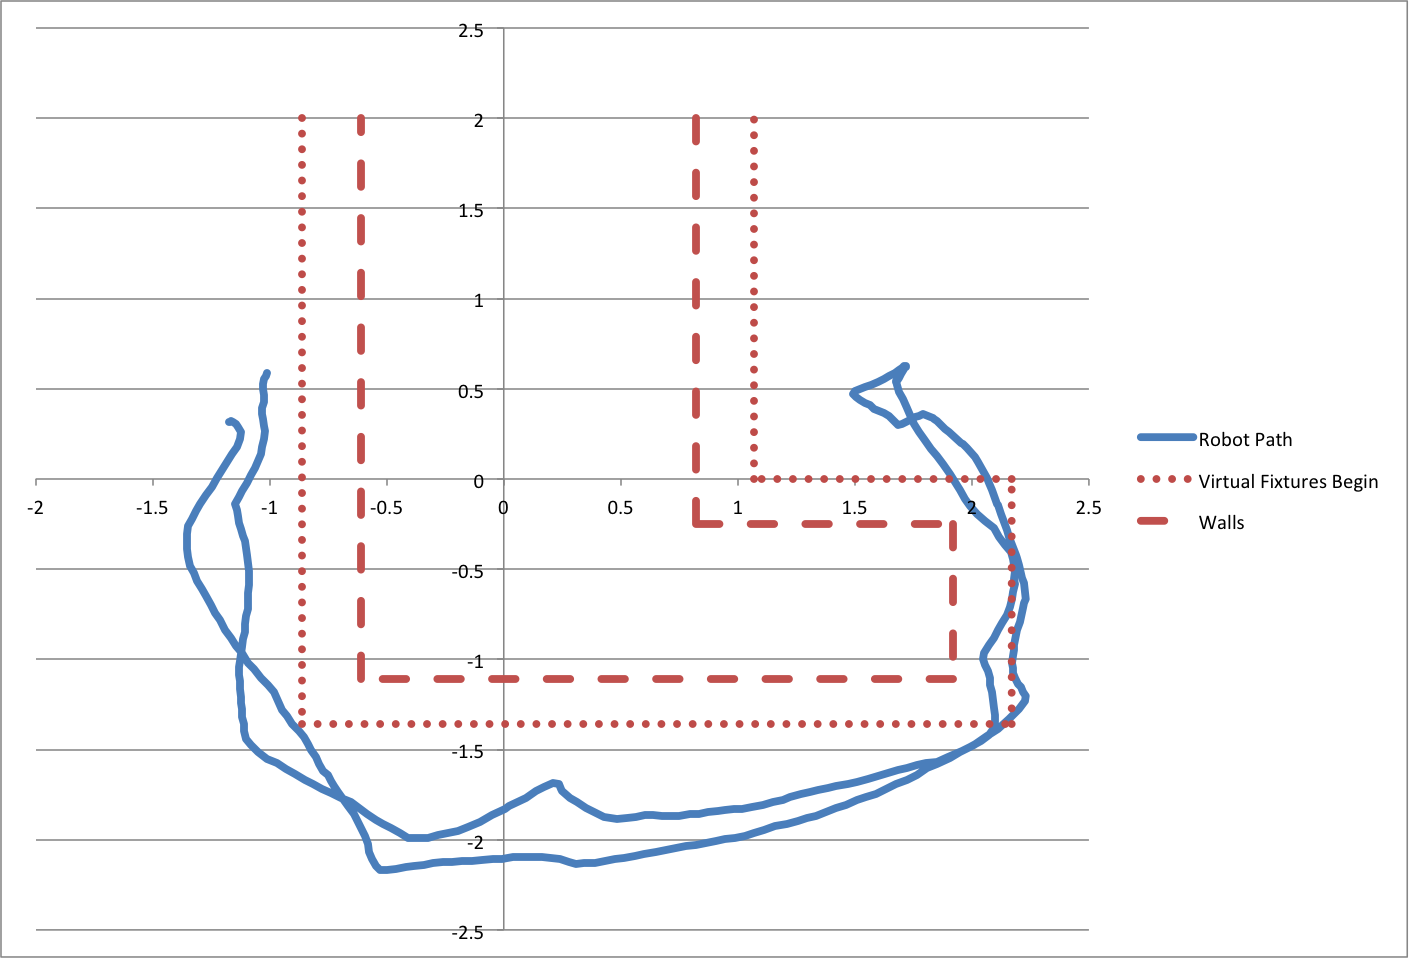
\includegraphics[width=0.8\textwidth]{goodrun.png}
    \caption{Example of a Test Run Using Virtual Fixtures}
    \label{fig:smooth}
\end{figure} 

On average, as well as in nine out of the ten test subjects, using the virtual fixture command strategy was faster than performing the task without virtual fixtures. The effectiveness and accuracy of the operator was determined by totalling the number of collisions and close calls. A collision is defined as more than 10\% of the Omnibot crossing the wall boundary, a close call is when the Omnibot crosses the wall boundary with less than 10\% of its frame. Due to a significant amount of backlash in the wheel-motor linkage and the configuration of the omni-wheels there is an unpredictability in the Omnibot's movement that can only be corrected to a certain extent using the on-board control system. Out of a total of one hundred test runs, there were nearly half as many crashes and close calls when using virtual fixtures compared to the runs without virtual fixtures. However, since the software will not allow the robot to move past a wall boundary, all the crashes and close calls that occurred during testing with virtual fixtures can be attributed to the mechanical drive properties of the robot base, mainly the travel of the wheels while the motors (and motor encoders) do not move. Though there were a number of collisions with the virtual fixture command strategy, a factor of safety can be implemented in the positioning of the virtual fixtures since the drive accuracy of the Omnibot only affects positioning to a limited amount.\\

Fig. \ref{fig:collisions} shows a test run without virtual fixtures. The operator, whether unintentionally, by choice, or through poor skills, drove across a wall boundary. In doing so they were able to complete the task slightly quicker, although in an environment with real walls in place of simulated walls they would have significantly damaged the robot. By avoiding unnecessary collisions the mobile robot will last longer and need less repairs, ultimately making the robot more cost-effective in its implementation.\\

Fig. \ref{fig:smooth} shows an example of a test run using virtual fixtures. At one point, the operator enters the region in which the virtual fixture can be felt, then navigates away to avoid a possible collision. Shortly after as the operator approaches the target location, they are able to closely pass by the wall corner with the knowledge that the command strategy will prevent them from accidentally coming too close and colliding with the wall. This knowledge allows the test subject to operate the robot with more confidence and less concern for damaging the robot, leading to a less stressful teleoperation experience.\\


\section{Conclusions}
\label{sec:con}

This work presented a novel command strategy that combines operator skill, haptic feedback, and a low level of autonomy to achieve teleoperation performance better than previously attainable using only a single input device. The haptic features of the joystick were utilized to further enhance teleoperation. As shown in the test results, operators were able to perform tasks faster and with better accuracy when using the novel command strategy. As well as completion time, a more critical aspect of teleoperation was improved, namely collisions. When driving the Omnibot base the operator was able to minimize undesirable movement and collisions. Further design changes on the robot test bed to minimize the drivetrain backlash will eliminate collisions entirely.\\

The main driving force behind this research is the consensus among mobile robot operators that the task of teleoperation is difficult and stressful. Since these are criteria that are very difficult to quantify, it is equally difficult to empirically demonstrate improvement in these areas. The best one can do is interview each test subject on their impressions of the command strategy. When asked about the novel command strategy presented, all operators agreed that the virtual fixtures made the task easier and less stressful. They were able to drive the robot with more confidence knowing the virtual fixtures would prevent them from collisions that may damage the robot. Based on test subject interviews and performance results, it can be concluded that the improved command strategy was a success.\\

\subsection{Future Work}

Since this command strategy was developed to be as multi-use as possible, there are many directions in which to take this research. The programming was written with customizability in mind, and therefore can be changed to suit specific tasks. With a particular task in mind, virtual fixtures can be added or modified to show an even more drastic improvement in operator performance for that task.\\

To carry on this research with the goal of keeping the command strategy useful for a variety of tasks, more challenging tests can be created to examine the merits of the virtual fixtures and command strategy. There are many variants of the virtual fixtures presented that can be tested, as well as types of virtual fixtures that have not yet been implemented. With the nearly endless variety and configurations of virtual fixtures, there is sure to be more research to come in the field of teleoperating mobile-manipulator systems using haptic devices. With the research presented herein, and that which is yet to be done, teleoperation will undoubtedly become easier, less stressful, more effective, and more efficient with the use of virtual fixtures in mobile robotics.\\

\section{Acknowledgements}

The authors would like to thank Cameco Corporation for their financial support of this work.\\

\bibliographystyle{asmems4}



\bibliography{asme2e}

\end{document}

